\documentclass[10pt,xcolor=pdflatex,dvipsnames,table]{beamer}
\usepackage{newcent}
\usepackage[utf8]{inputenc}
\usepackage[czech]{babel}
\usepackage{hyperref}
\usepackage{amsthm}
\usepackage{amssymb}
\usepackage{amsmath}
\usepackage{array}
\usepackage{stmaryrd}
\usepackage{graphicx}
\usepackage{tabularx}
\usepackage{listings}
\usepackage{fancyvrb}
\usepackage{minted}
\usepackage{multicol}
%\usepackage{packages/beamerthemeFIT}

\makeatletter
  \def\beamer@calltheme#1#2#3{%
    \def\beamer@themelist{#2}
    \@for\beamer@themename:=\beamer@themelist\do
    {\usepackage[{#1}]{\beamer@themelocation/#3\beamer@themename}}}

  \def\usefolder#1{
    \def\beamer@themelocation{#1}
  }
  \def\beamer@themelocation{}

\usefolder{packages}
\usetheme{FIT}



\title[OpenGL]{PGR - Fragment Shader, Světlo, Barvy,}

\author[]{Tomáš Milet}

\institute[]{Brno University of Technology, Faculty of Information Technology\\
Bo\v{z}et\v{e}chova 1/2. 612 66 Brno - Kr\'alovo Pole\\
imilet@fit.vutbr.cz}

\date{\today}

\begin{document}

\frame[plain]{\titlepage}

\setbeamercolor{background canvas}{bg=fitblue}
\begin{frame}
\frametitle{Color / Barva}
\begin{center}
\Huge {\color{white}Color / Barva}
\end{center}
\end{frame}
\setbeamercolor{background canvas}{bg=white}


\begin{frame}
    \frametitle{Color / Barva}
    \begin{columns}[c]
    \column{.5\textwidth}
        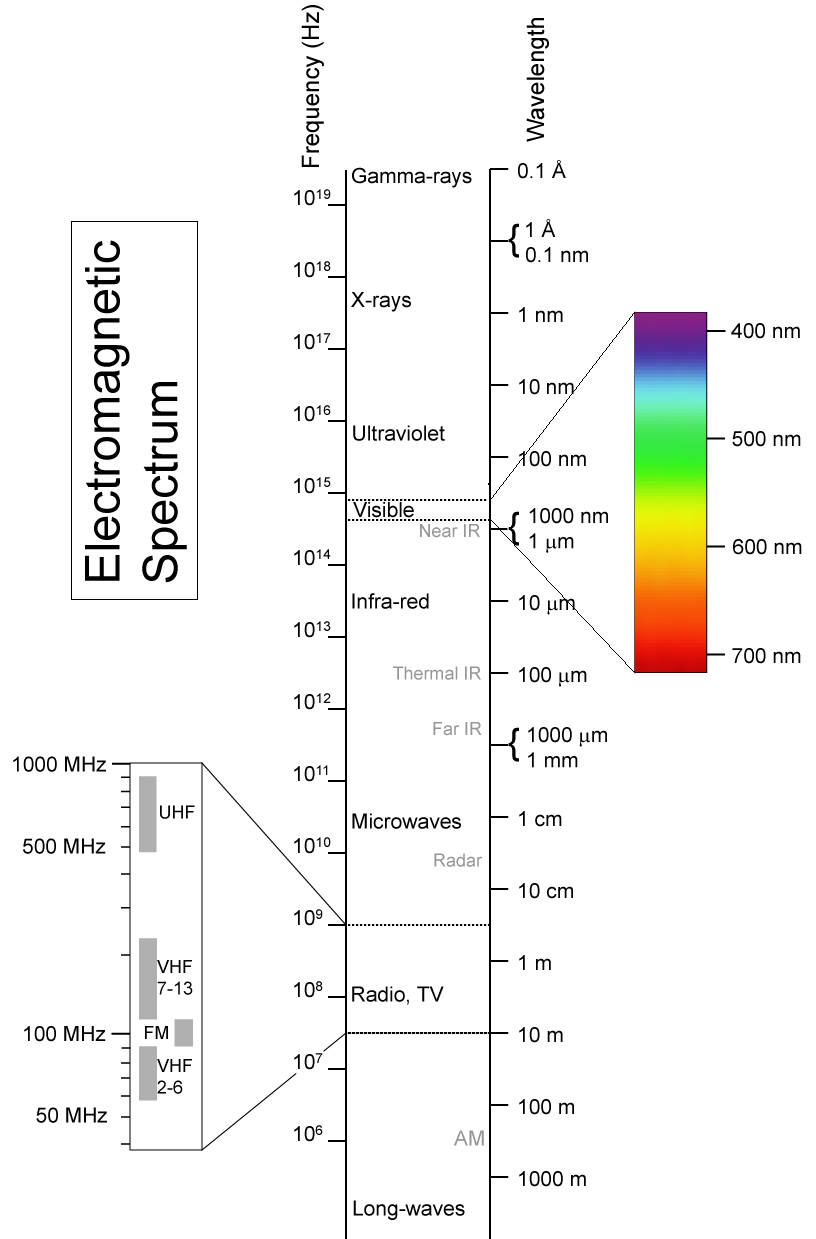
\includegraphics[height=\textheight]{pics/color/Electromagnetic-Spectrum}
    \column{.5\textwidth}
        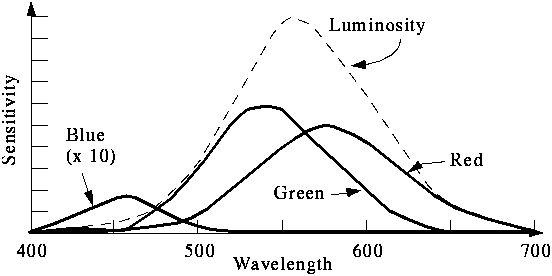
\includegraphics[width=\textwidth]{pics/color/citlivost-oka}

        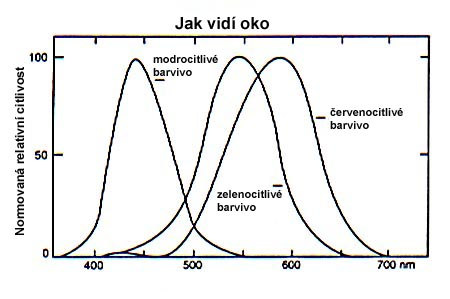
\includegraphics[width=\textwidth]{pics/color/citlivost-oka-normovana}
    \end{columns}
\end{frame}

\begin{frame}
    \frametitle{Gamut}
    \begin{columns}[c]
    \column{.5\textwidth}
        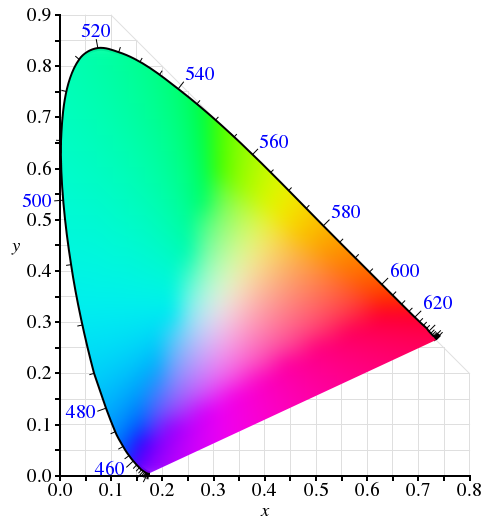
\includegraphics[width=\textwidth]{pics/color/gamut}
    \column{.5\textwidth}
        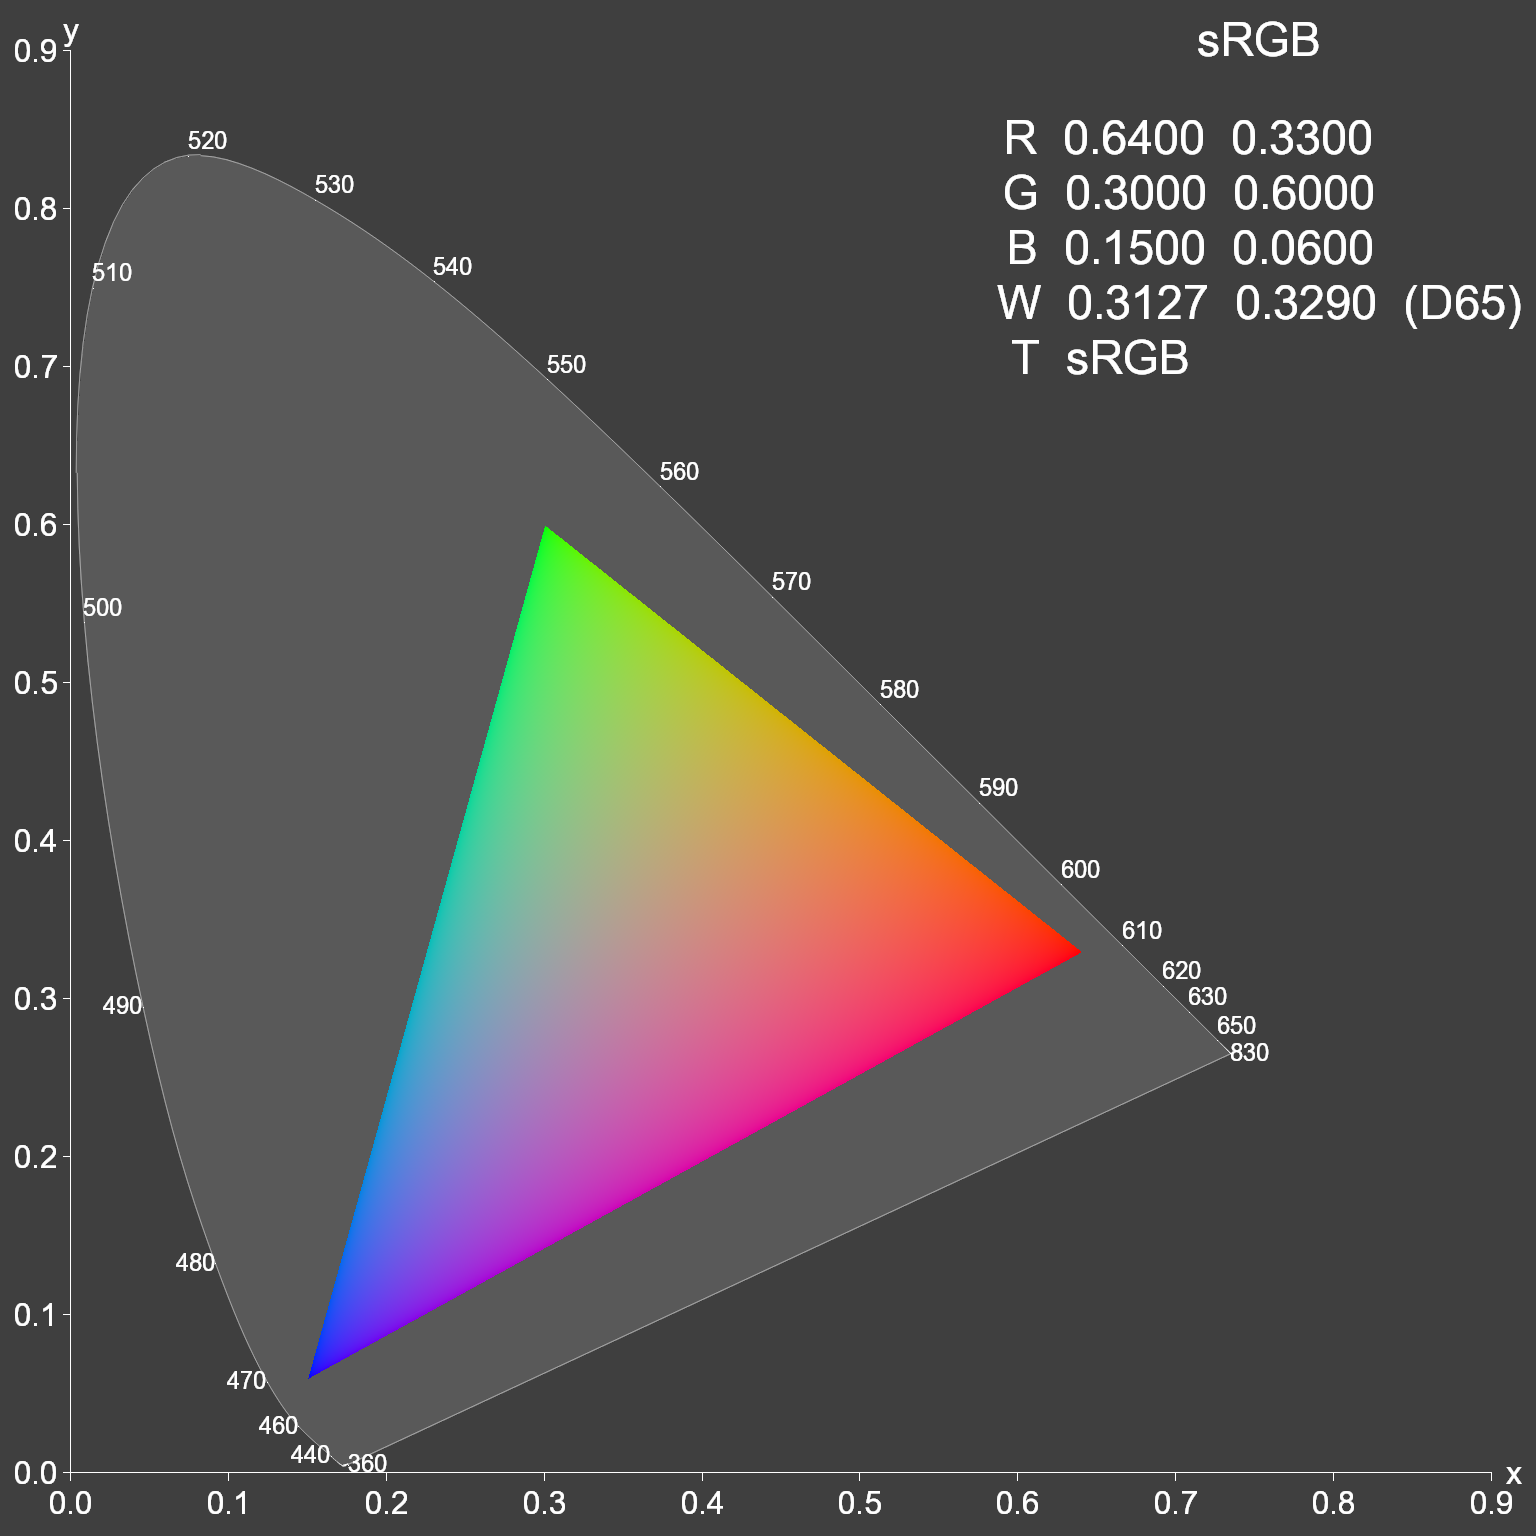
\includegraphics[width=\textwidth]{pics/color/Gamut-sRGB}
    \end{columns}
    \vfill
    \begin{itemize}
        \item CIE 1931
        \item XYZ vs RGB
    \end{itemize}
\end{frame}

\begin{frame}
    \frametitle{Gamma}

    \begin{columns}[c]
    \column{.5\textwidth}
        \scriptsize
        Logarithmic sensitivity of human eye\\
        Logaritmická citlivost oka

        \begin{eqnarray*}
        C_\mathrm{srgb}=\begin{cases}
        12.92C_\mathrm{l}, & C_\mathrm{l} \le t\\
        (1+a)C_\mathrm{l}^{\frac{1}{2.4}}-a, & C_\mathrm{l} > t
        \end{cases} \\
        a = 0.055 \\
        t = 0.0031308
        \end{eqnarray*}
        
    \column{.5\textwidth}
        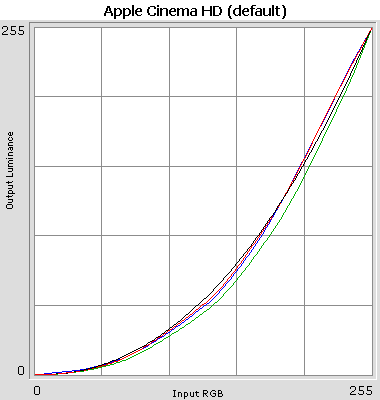
\includegraphics[width=\textwidth]{pics/color/monitor}
    \end{columns}
\end{frame}

\begin{frame}[fragile]
    \frametitle{Colors in OpenGL / Barva v OpenGL}

    Pipeline :
    \begin{itemize}
        \item float RGB(A) (vec3)
        \item {\color{black}$(0,0,0)$ \color{red}$(1,0,0)$ \color{green}$(0,1,0)$ \color{blue}$(0,0,1)$}
        \item[\color{red}!] Linear Color space, interpolation, blending.
    \end{itemize}
    \pause\vfill
    Vstupy a framebuffer :
    \begin{itemize}
        \item The most common RGB8
        \item Others : RGB16, RGB565, ...
        \item Linear or sRGB
        \item Conversion by hand?
    \end{itemize}
\begin{minted}[bgcolor=bg]{packages/c_cpp.py:CppLexer -x}
//default framebuffer
SDL_GL_SetAttribute(SDL_GL_FRAMEBUFFER_SRGB_CAPABLE,1);
...
//enabling SRGB in OpenGL
glEnable(GL_FRAMEBUFFER_SRGB);
\end{minted}
\end{frame}

\begin{frame}[fragile]
\frametitle{Gamma Correct}
  \scriptsize
	\begin{itemize}
  \item The light computation has to be done in linear space.
  \item After the computation is done, it has to be gamma corrected.
  \item Sharp transition from lit and shadowed parts.
	\end{itemize}
	\begin{itemize}
  \item Výpočet osvětlení musí být proveden v lineárním prostoru.
  \item Po výpočtu osvětlení je nutné obrázek upravit gamma korekcí.
  \item Ostrý přechod ze světla do stínu je správně.
	\end{itemize}
	\begin{figure}[h]
	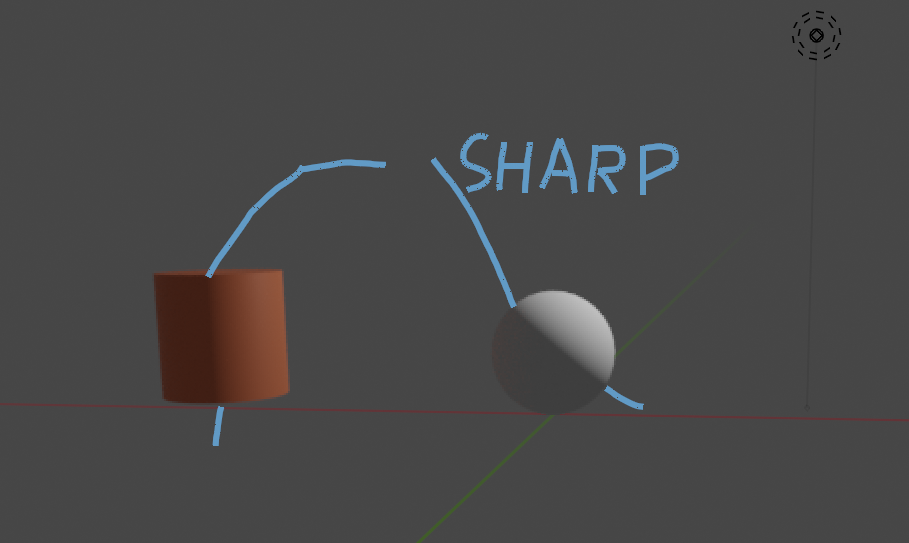
\includegraphics[width=8cm,keepaspectratio]{pics/color/gamma_correct}
	\end{figure}
\end{frame}

\begin{frame}[fragile]
\frametitle{Real Image}
	\begin{figure}[h]
	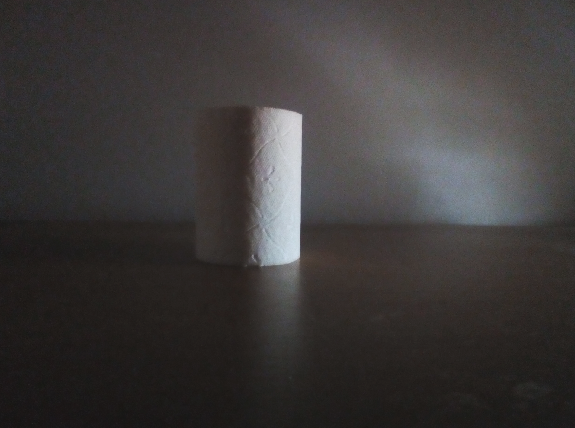
\includegraphics[width=8cm,keepaspectratio]{pics/color/gamma_real}
	\end{figure}
\end{frame}

\begin{frame}[fragile]
\frametitle{Gamma Correct}
	\begin{itemize}
  \item Left incorrect, right correct.
	\end{itemize}
	\begin{itemize}
  \item Vlevo bez korekce, vpravo s korekcí.
	\end{itemize}
	\begin{picture}(120,150)
		\put(0,0){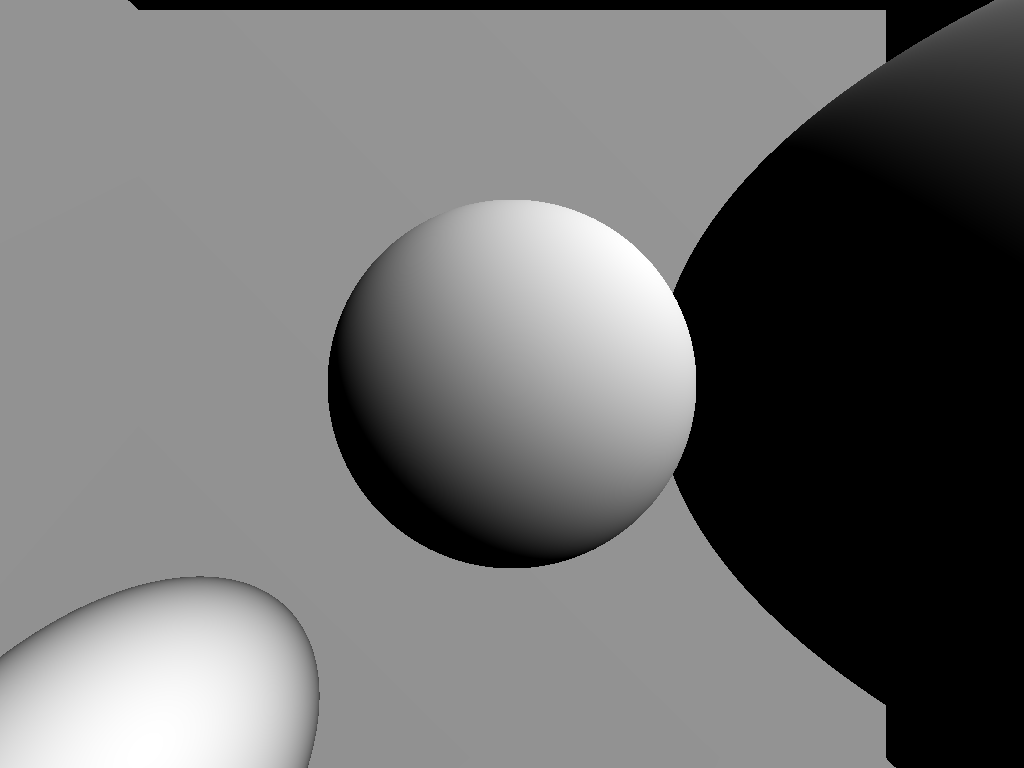
\includegraphics[width=6cm,keepaspectratio]{pics/color/no_correction}}
	\end{picture}
	\begin{picture}(60,40)
		\put(50,0){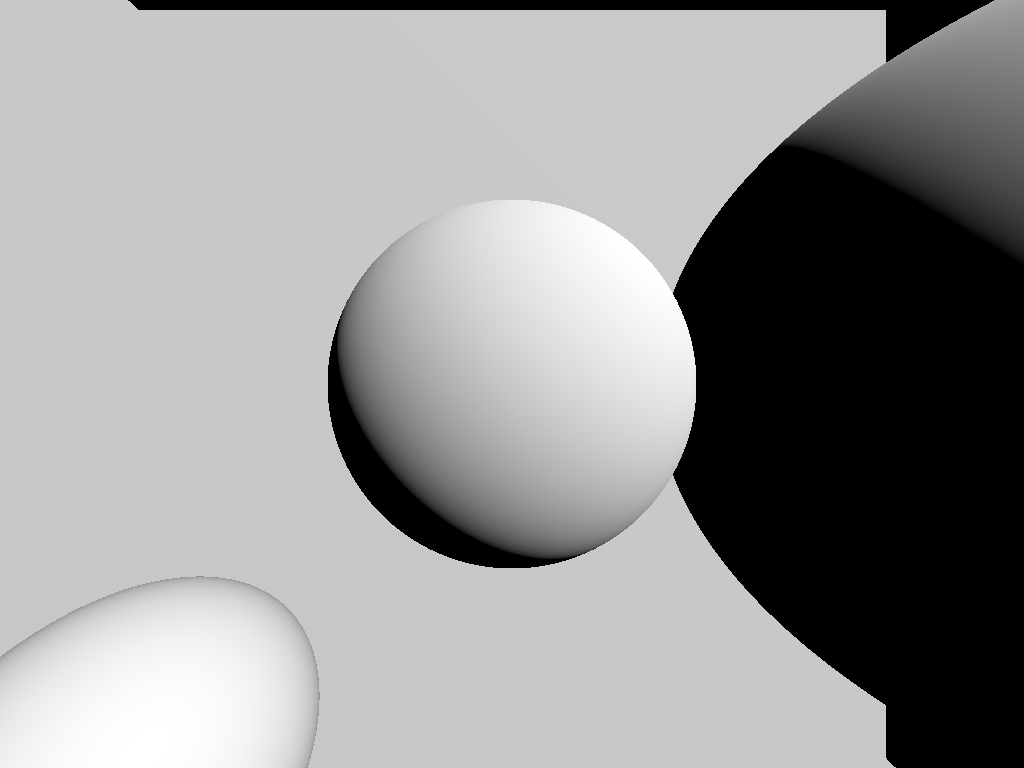
\includegraphics[width=6cm,keepaspectratio]{pics/color/correction}}
	\end{picture}
\end{frame}

\setbeamercolor{background canvas}{bg=fitblue}
\begin{frame}
\frametitle{Light-Matter Interaction / Interakce světla a hmoty}
\begin{center}
\Huge {\color{white}Light-Matter Interaction / Interakce světla a hmoty}
\end{center}
\end{frame}
\setbeamercolor{background canvas}{bg=white}

\begin{frame}
  \scriptsize
  \begin{itemize}
    \item Three kinds of interactions: Absorption, Scattering, Emission.
  \end{itemize}
  \begin{itemize}
    \item Tři druhy interakcí: Pohlcení, odraz/lom, vyzáření.
  \end{itemize}
  \frametitle{Absoption, scattering}
  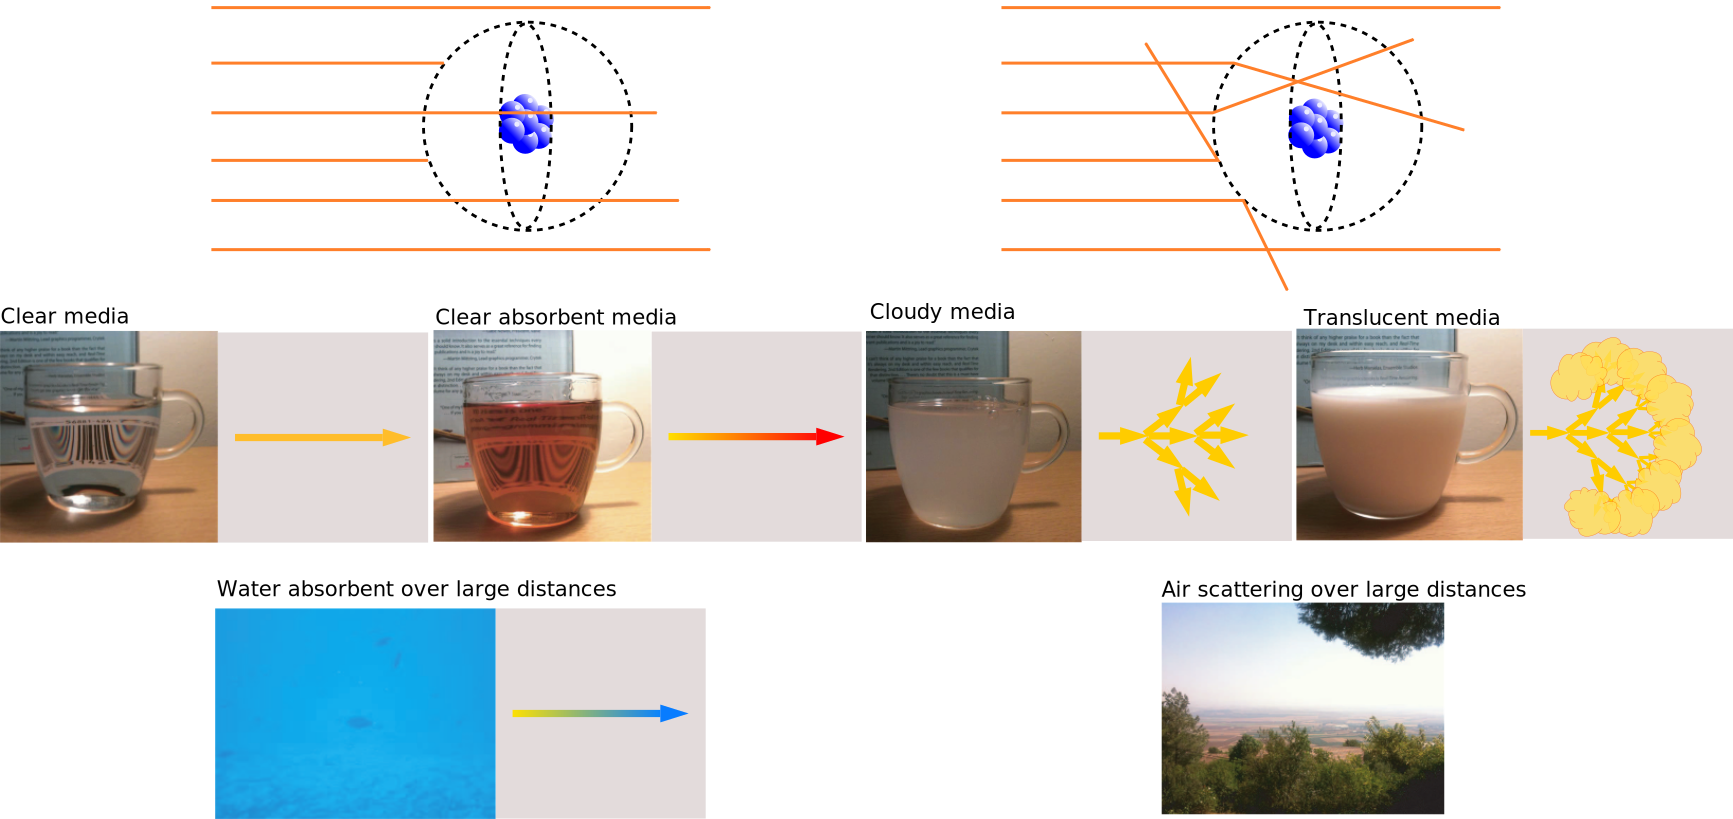
\includegraphics[width=\textwidth]{pics/physicallyBasedRendering/scattering_absorption2/scattering_absorption}
\end{frame}

\begin{frame}\frametitle{Absoption, scattering}
  \scriptsize
  \begin{itemize}
    \item Absorption and scattering are semi independent values.
    \item But fotons that are absorbed cannot be scattered.
    \item And fotons that are scattered cannot be absorbed.
  \end{itemize}
  \begin{itemize}
    \item Absorpce a odraz jsou více méně nezávislé hodnoty.
    \item Ale fotony, které jsou absorbovány nemůžou být odraženy a naopak.
  \end{itemize}
  \begin{figure}[ht]
  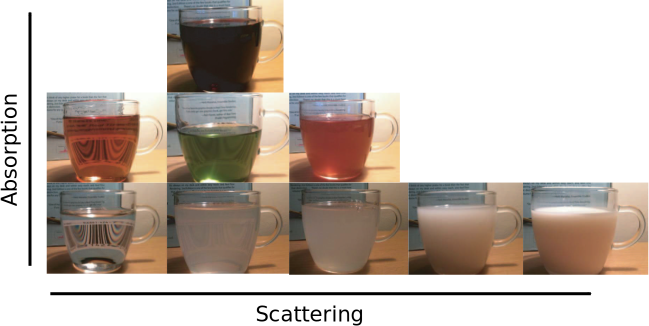
\includegraphics[width=0.8\textwidth]{pics/physicallyBasedRendering/scattering_absorption1/scattering_absorption}
  \end{figure}
\end{frame}

\begin{frame}\frametitle{Specular, diffuse component}
  \scriptsize
  \begin{itemize}
    \item Specular component is a light directly reflected from a surface.
    \item Specular component is dominant in metals.
    \item Diffuse component is dominant in dielectrics/isolants.
    \item Diffuse component is a light scattered inside material, when the entry and exit point of the light is closer than the size of screen pixel.
  \end{itemize}
  \begin{itemize}
    \item Spekulární složka je odražené světlo přímo z povrchu.
    \item Je dominantní pro kovy.
    \item Difuzní složka je dominantní pro dielektrika / izolanty.
    \item Je to světlo, které se zalomilo uvnitř materiálů. Vstup světla a výstup světla z materiálu musí být k sobě blíž než je velikost pixelu.
  \end{itemize}
  \begin{figure}[ht]
  
\includegraphics[width=0.5\textwidth]{pics/physicallyBasedRendering/specular_diffuse}
  \end{figure}
\end{frame}

\begin{frame}\frametitle{Subsurface scattering}
  \scriptsize
  \begin{itemize}
    \item If the entry and exit point of the light is far away from each other, we are talking about subsurface scattering not about diffuse light.
    \item Wax, skin, ...
  \end{itemize}
  \begin{itemize}
    \item Když jsou vstupní a výstupní body světla od sebe daleko, mluvíme od pod povrchovém lomení světla. Řeší se pomocí jiných metod.
    \item Vosk, kůže, ...
  \end{itemize}
  \begin{figure}[ht]
  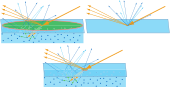
\includegraphics[width=0.6\textwidth]{pics/physicallyBasedRendering/subsurface_pixel_size}
  \end{figure}
\end{frame}

\begin{frame}\frametitle{Metals / Lom světla kovů}
  \scriptsize
  \begin{itemize}
    \item Metals only reflect incoming light or convert the light to other forms of energy.
    \item Left: metal, right: non-metal
  \end{itemize}
  \begin{itemize}
    \item Kovy světlo pouze odráží nebo přeměňují na jiný druh energie (teplo).
    \item Vlevo: kov, vpravo: nekov
  \end{itemize}
  \begin{figure}[ht]
    
\includegraphics[width=\textwidth]{pics/physicallyBasedRendering/metal_refraction}
  \end{figure}
\end{frame}

\begin{frame}\frametitle{Surface roughness and microfacets / Drsnost povrchu a mikroplošky}
  \scriptsize
  \begin{itemize}
    \item Microscopic structures determine coherency of reflected light rays.
    \item Microfacet distribution determines the clarity of mirror images.
  \end{itemize}
  \begin{itemize}
    \item Mikroskopické struktury určují koherentnost odražených paprsků.
    \item Distribuce mikroplošek určuje čistost zrcadlového odrazu.
  \end{itemize}
  \begin{figure}[ht]
    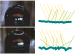
\includegraphics[width=0.5\textwidth]{pics/physicallyBasedRendering/roughness/roughness.pdf}
  \end{figure}
\end{frame}

\begin{frame}\frametitle{Microfacet shadowing / Zastínění mikroplošek}
  
\includegraphics[width=\textwidth]{pics/physicallyBasedRendering/microfacets_occlusion}
\end{frame}

\begin{frame}\frametitle{Microfacet shadowing / Zastínění mikroplošek}
  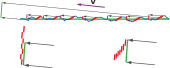
\includegraphics[width=\textwidth]{pics/physicallyBasedRendering/microfacet_masking}
\end{frame}

\begin{frame}\frametitle{State of the art}
  \begin{figure}[ht]
    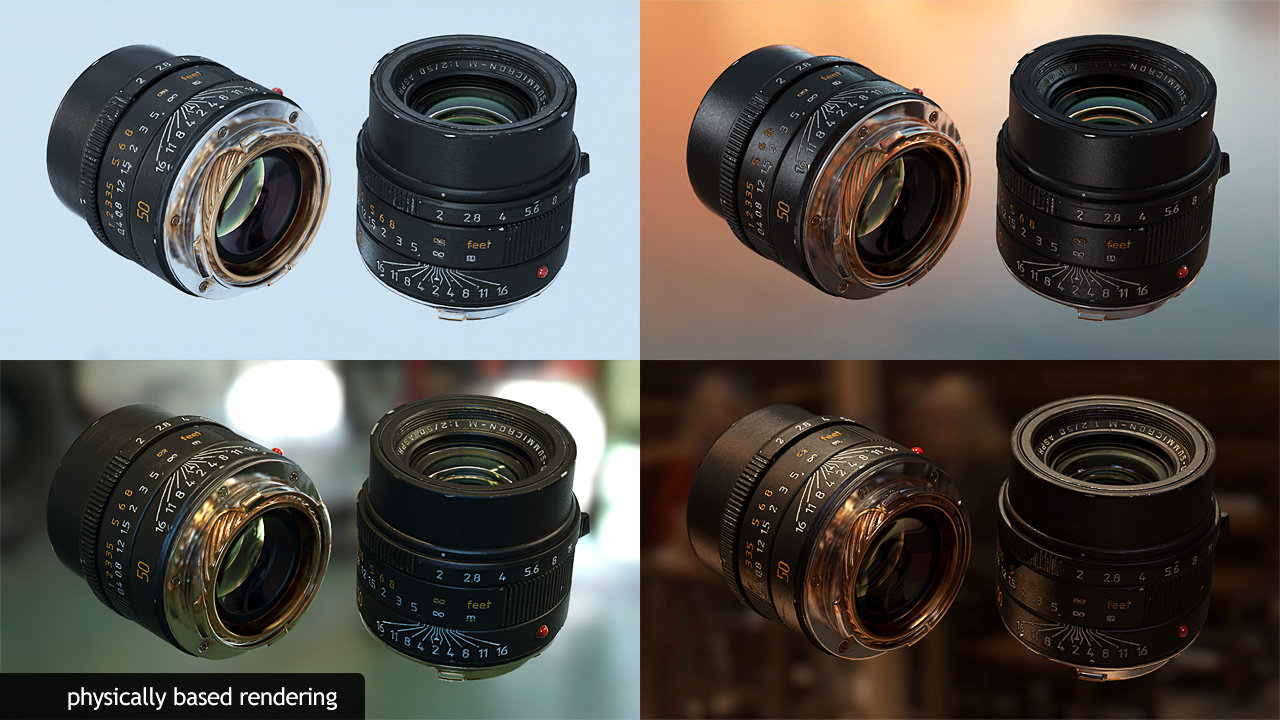
\includegraphics[width=0.8\textwidth]{pics/physicallyBasedRendering/pbr}
  \end{figure}
\end{frame}

\begin{frame}\frametitle{Metalic workflow}
  \begin{columns}[c]
  \column{.5\textwidth}
    \scriptsize
    \begin{itemize}
      \item Metalic workflow is intuitive way of representing different material properties.
      \item Color, metalness, roughness, normals.
      \item Metalness 1 or 0: metal or non-metal.
      \item Roughness represents microfacets.
    \end{itemize}
    \begin{itemize}
      \item Metalická reprezentace materiálů je intuitivní.
      \item Barva, kovovost, drsnost, a normálová mapa.
      \item Metalness (kovovost) je buď jedna nebo nula.
      \item Roughness (drsnost) předtavuje distribuci mikroplošek.
    \end{itemize}
  \column{.5\textwidth}
    
\includegraphics[width=0.48\textwidth]{pics/physicallyBasedRendering/metal/color}
    
\includegraphics[width=0.48\textwidth]{pics/physicallyBasedRendering/metal/metalness}
    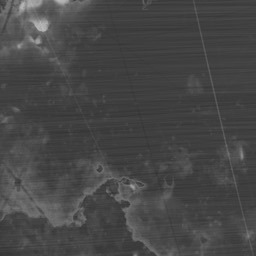
\includegraphics[width=0.48\textwidth]{pics/physicallyBasedRendering/metal/roughness}
    
\includegraphics[width=0.48\textwidth]{pics/physicallyBasedRendering/metal/normal}
  \end{columns}
\end{frame}

\begin{frame}\frametitle{Metalness and roughness}
  \scriptsize
  \begin{itemize}
    \item Top row: Non-metal, bottom row: metal.
    \item From left to right: roughness from 0 to 1
  \end{itemize}
  \begin{itemize}
    \item Horní řádek nekov, dolní kov.
    \item Zleva do prava, zvyšující se drsnost od 0 po 1. 
  \end{itemize}
  \begin{figure}[ht]
    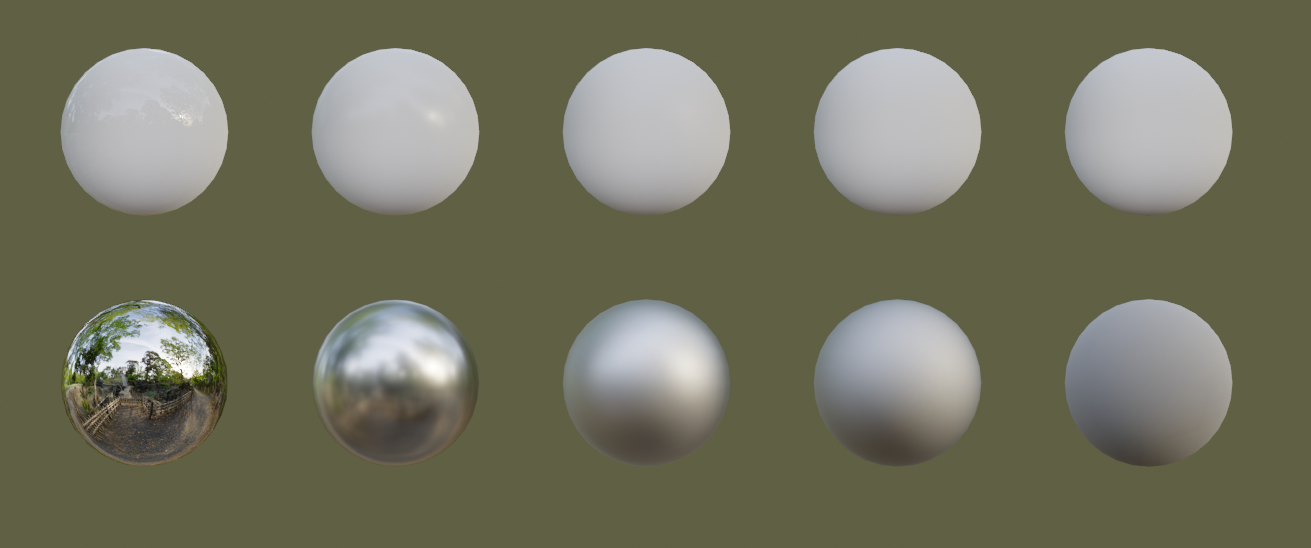
\includegraphics[width=\textwidth]{pics/physicallyBasedRendering/metal/roughness_metalness}
  \end{figure}
\end{frame}

\begin{frame}\frametitle{Normal map}
  \scriptsize
  \begin{itemize}
    \item Left: without normal map, Right: with normal map
  \end{itemize}
  \begin{itemize}
    \item Vlevo: bez normálové mapy, vpravo s normálovou mapou
  \end{itemize}
  \begin{figure}[ht]
    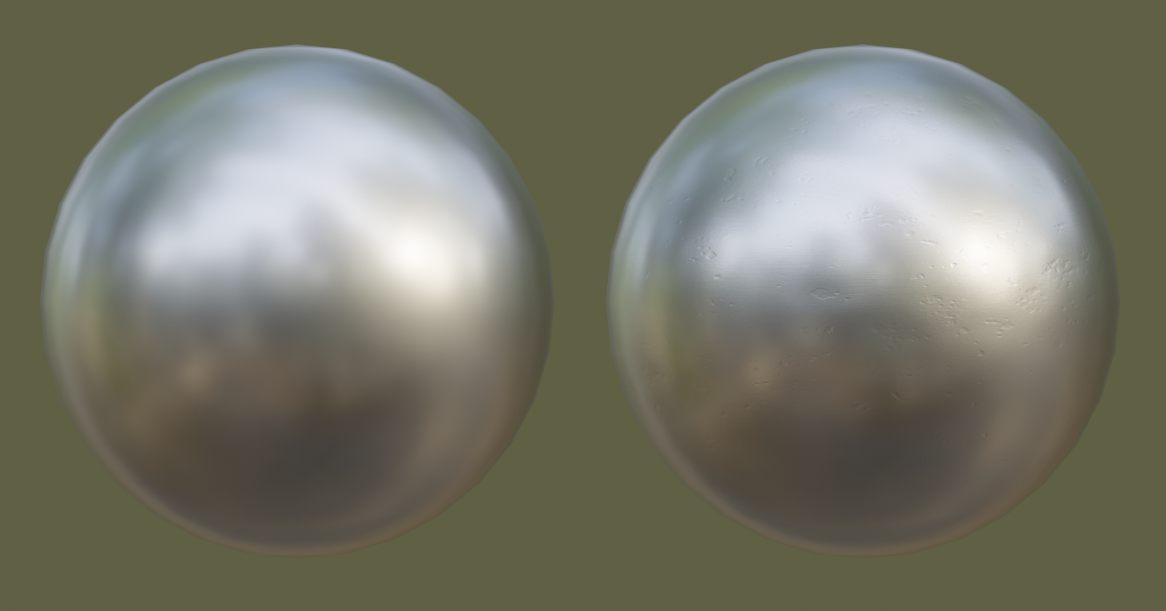
\includegraphics[width=\textwidth]{pics/physicallyBasedRendering/metal/normal_map}
  \end{figure}
\end{frame}

\begin{frame}\frametitle{Environment mapping}
  \scriptsize
  \begin{figure}[ht]
    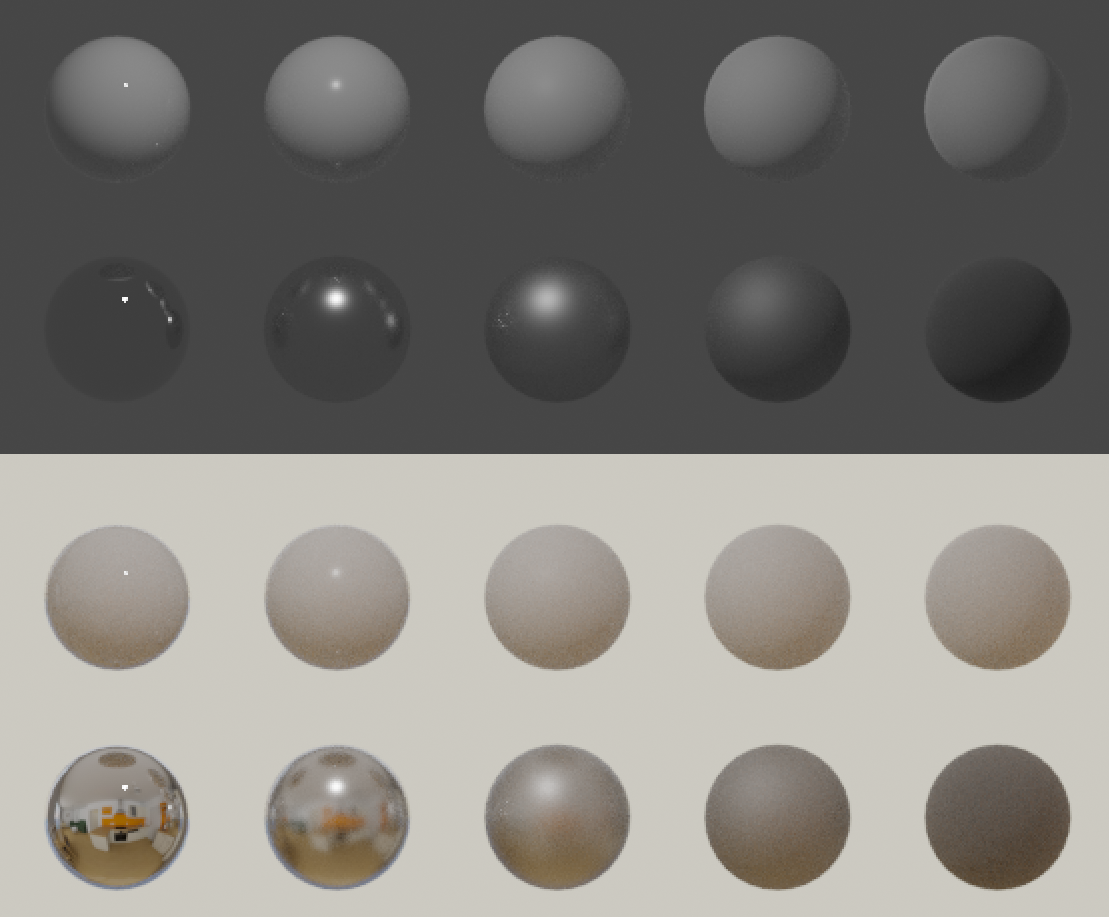
\includegraphics[width=0.5\textwidth]{pics/physicallyBasedRendering/metal/environment_map}
  \end{figure}
\end{frame}

\begin{frame}\frametitle{Metalic workflow}
  \begin{figure}[ht]
    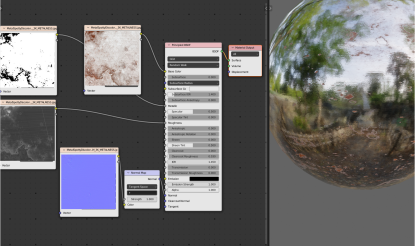
\includegraphics[width=\textwidth]{pics/physicallyBasedRendering/metal/metal_workflow}
  \end{figure}
\end{frame}

\begin{frame}
    \frametitle{Illumination / Osvětlení}

    \begin{columns}[c]
    \column{.5\textwidth}

    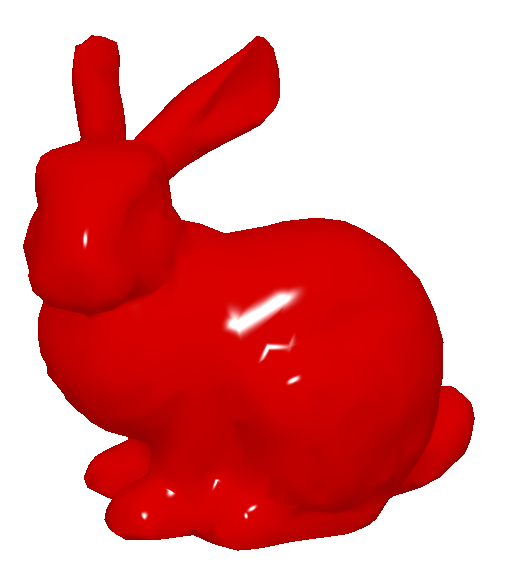
\includegraphics[width=\textwidth]{pics/physicallyBasedRendering/bunny}

    \column{.5\textwidth}

    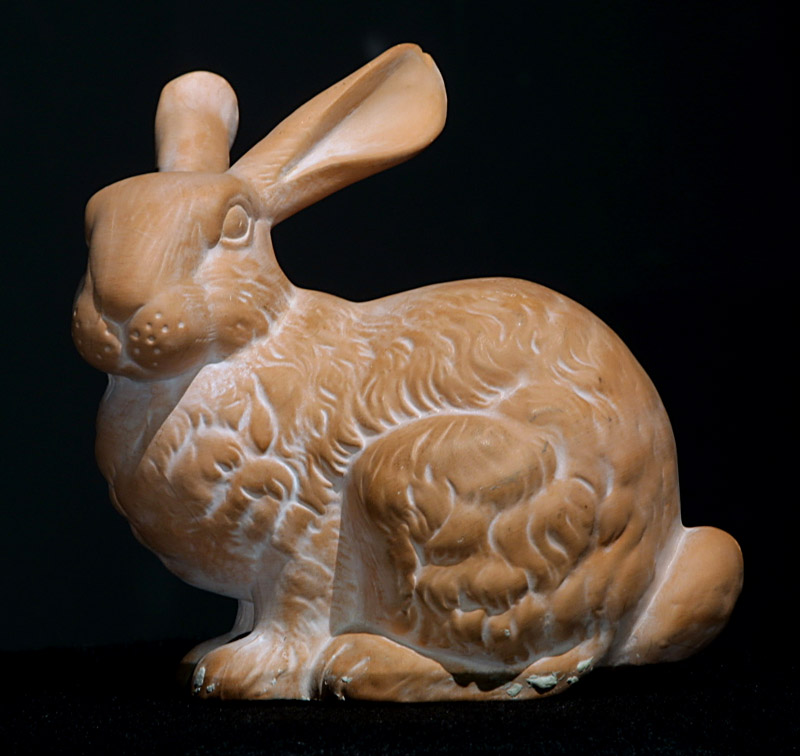
\includegraphics[width=\textwidth]{pics/physicallyBasedRendering/stanford-bunny}
    
    \end{columns}
\end{frame}

\begin{frame}
    \frametitle{Rendering equation / Zobrazovací rovnice}
    \begin{equation*}
        L_o(\mathbf x, \omega, \lambda, t) = L_e(\mathbf x, \omega, \lambda, t) + \int\limits_\Omega f_r(\mathbf x, \omega', \omega, \lambda, t) L_i(\mathbf x, \omega', \lambda, t) (-\omega' \cdot \mathbf n) d \omega'
    \end{equation*}
    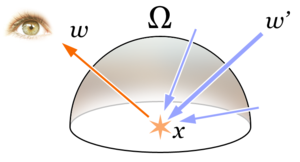
\includegraphics[width=2in]{pics/physicallyBasedRendering/rendering}
    \vfill
    Siggraph 1986 :
    \begin{equation*}
        \displaystyle I(x, x') = g(x, x')\left[ e(x, x') + \int\limits_S p(x, x', x'')I(x', x'')dx''\right]
    \end{equation*}
\end{frame}

\begin{frame}\frametitle{Local illumination models / Lokální osvětlovací model}
  \scriptsize
  \begin{itemize}
      \item Light reflection in "one point"
      \item Differential scene surface.
  \end{itemize}
  \begin{itemize}
      \item Odraz světla v "jednom bodu".
      \item Diferenciální ploška scény.
  \end{itemize}
  \pause\vfill
  \begin{equation*}
      L_{\{o,e,i\}}(\mathbf x, \omega, \lambda, t)
  \end{equation*}
  \begin{itemize}
       \item Radiance
       \item $W \cdot sr^{-1} \cdot m^{-2} (\cdot m^{-1})$
  \end{itemize}
  \pause\vfill
  \begin{equation*}
      f_r(\mathbf x, \omega', \omega, \lambda, t)
  \end{equation*}
  \begin{itemize}
      \item BRDF
      \item $sr^{-1}$
  \end{itemize}
\end{frame}

\begin{frame}\frametitle{BRDF}
  \scriptsize
  \begin{itemize}
      \item Bidirectional Reflectance Distribution Function.
      \item Almost like probability density function (pdf).
  \end{itemize}
  \begin{itemize}
      \item Bidirectional Reflectance Distribution Function.
      \item Hustota pravděpodobnosti (skoro).
  \end{itemize}
  \pause\vfill
  Reciprocity\\
  Reciprocita
  \begin{equation*}
      f_r(\mathbf x, \omega', \omega) = f_r(\mathbf x, \omega, \omega')
  \end{equation*}
  Conservation of energy\\
  Zákon zachování energie
  \begin{equation*}
      \int\limits_\Omega f_r(\mathbf x, \omega', \omega) (\omega \cdot \mathbf n) d\omega \le 1
  \end{equation*}
  Izotropy x Anisotropy\\
  Izotropie x Anizotropie
\end{frame}

\begin{frame}\frametitle{BRDF variants / Varianty BRDF}
  \begin{itemize}
    \item Phong
    \item Blinn-Phong
    \item Cook-Torrance
    \item GGX (microfacet distribution)
    \item ...
  \end{itemize}
  \pause\vfill
  \begin{itemize}
    \item Pragmatic x Physically Based
    \item Depends on Application.
  \end{itemize}
\end{frame}

\section{Light Reflection / Odraz světla}

\begin{frame}\frametitle{Odraz a lom světla}
  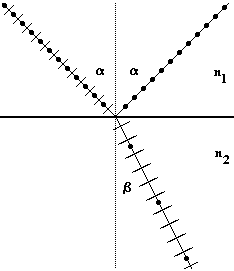
\includegraphics[width=.3\textwidth]{pics/physicallyBasedRendering/image106}
  \scriptsize
  \begin{itemize}
    \item Reflection and refraction happens on interface between two mediums.
    \item Index of Refraction (IOR) (light speed in the medium).
    \item Reflection based light polarization.
  \end{itemize}
  \begin{itemize}
    \item Odraz a lom na hranicích prostředí.
    \item Indexy lomu (rychlost v daném prostředí).
    \item Polarizace odrazem.
  \end{itemize}
  \begin{equation*}
    \frac{v_1}{v_2} = \frac{\sin\alpha}{\sin\beta}
  \end{equation*}
\end{frame}

\begin{frame}
    \frametitle{Energie}
    Fresnellovy vzorce
    \begin{equation*}
        R_s = \left| \frac{Z_2 \cos \theta_i - Z_1 \cos \theta_t}{Z_2 \cos \theta_i + Z_1 \cos \theta_t} \right|^2
    \end{equation*}
    \begin{itemize}
        \item Závislé na polarizaci.
        \item Nepraktické.
    \end{itemize}
    \pause\vfill
    Schlickova aproximace
    \begin{equation*}
        R(\theta) = R_0 + (1-R_0)(1-\cos\theta)^5
    \end{equation*}
    \begin{itemize}
        \item $R_0$ je vlastnost materiálu.
        \item Pro izolanty $R_0 \approx 0.04$.
        \item $\cos\theta \rightarrow 0$ ... $R \rightarrow 1$
    \end{itemize}
\end{frame}

\begin{frame}
    \frametitle{Fresnel reflectance}
    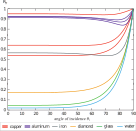
\includegraphics[width=0.5\textwidth]{pics/physicallyBasedRendering/fresnel_reflectance}
\end{frame}

\begin{frame}
    \frametitle{Fresnel reflectance}
    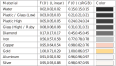
\includegraphics[width=0.8\textwidth]{pics/physicallyBasedRendering/fresnel_reflectance_table}
\end{frame}

\begin{frame}
    \frametitle{Nedokonalý povrch}
    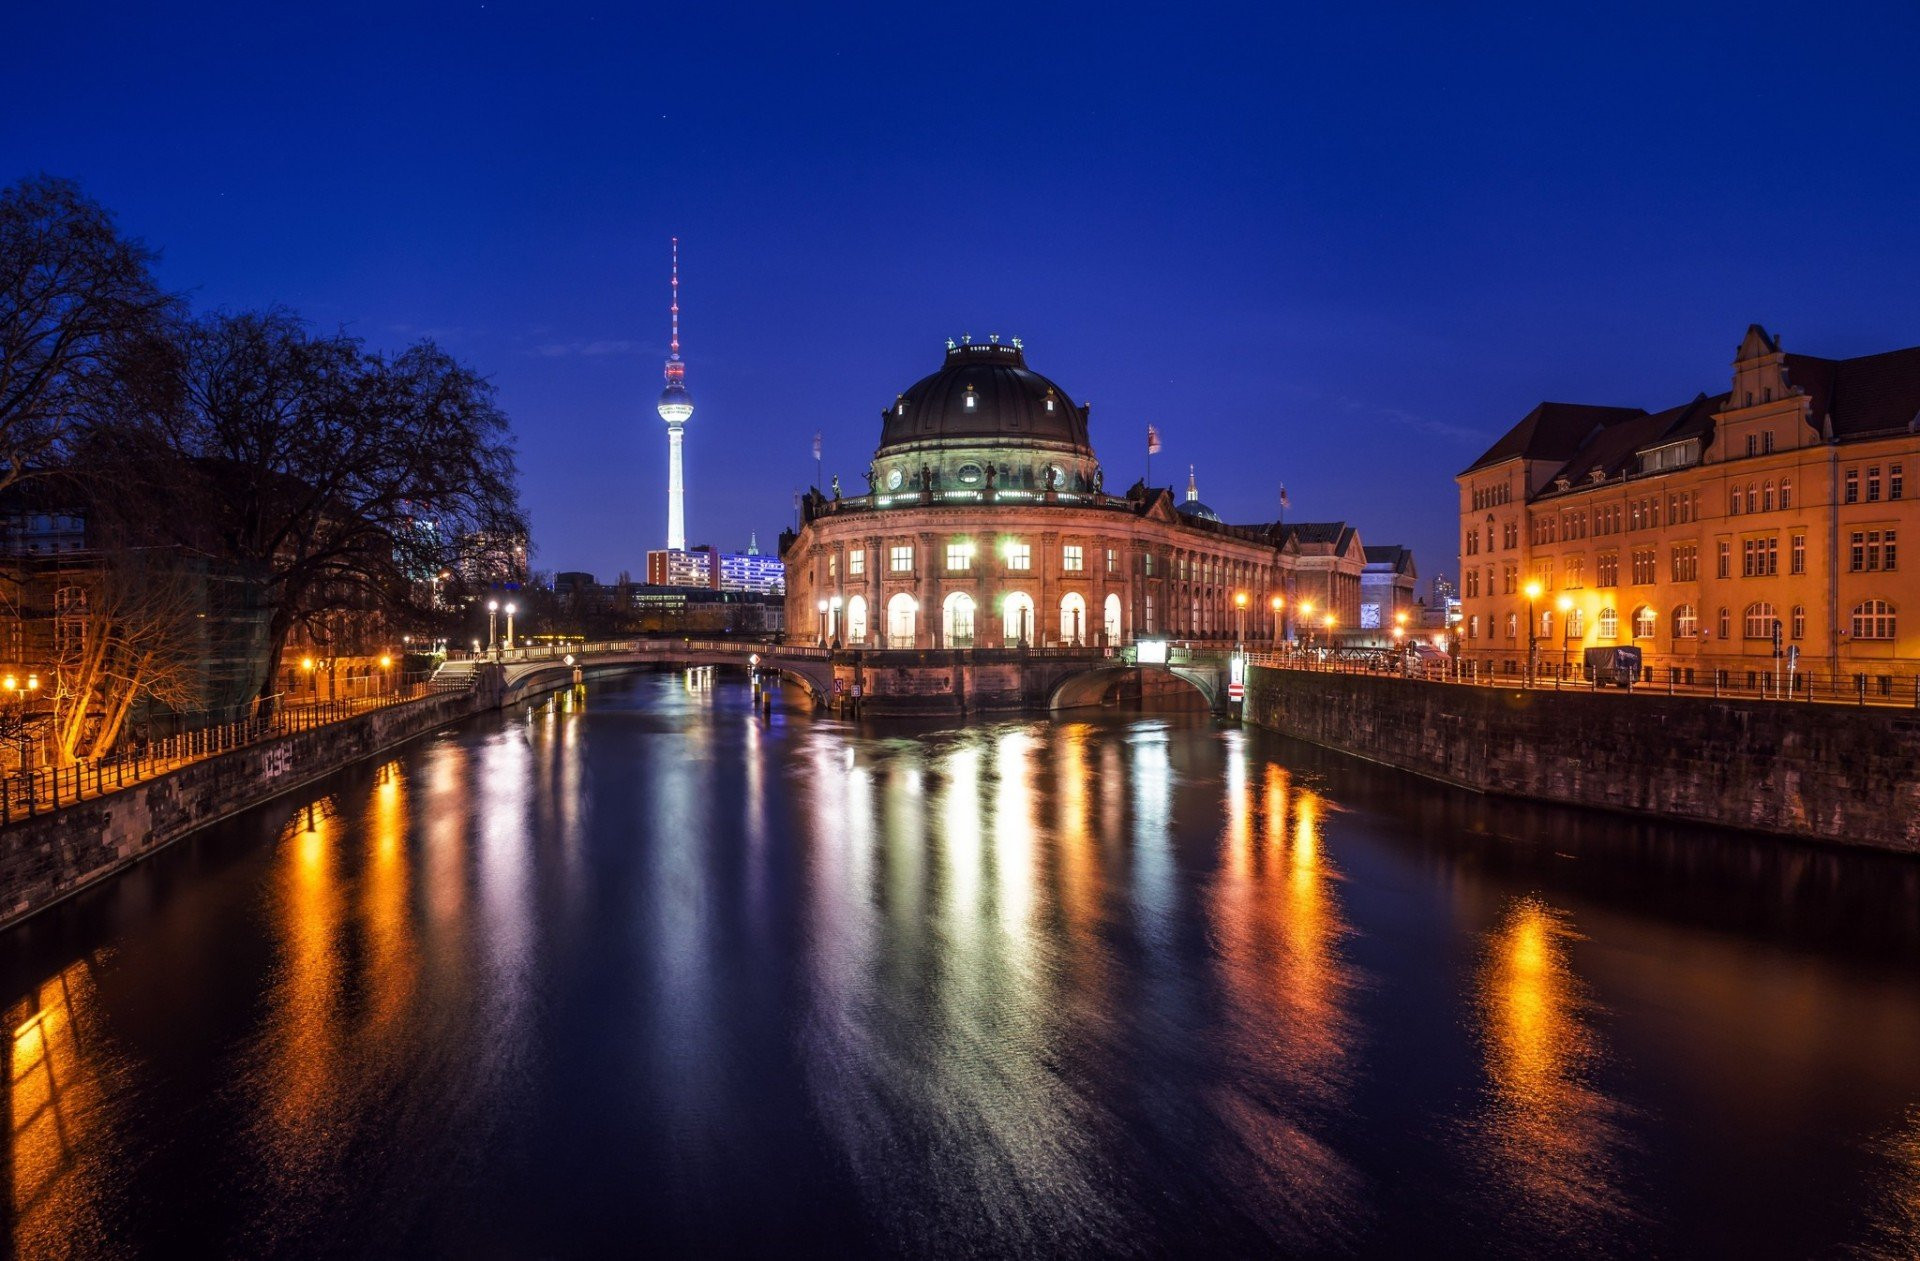
\includegraphics[width=0.8\textwidth]{pics/physicallyBasedRendering/night-reflect}
\end{frame}

\begin{frame}
    \frametitle{Mikroploškový model}

    \begin{columns}[c]
    \column{.5\textwidth}
    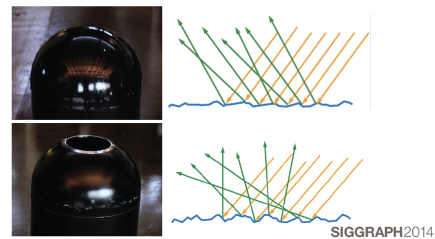
\includegraphics[width=\textwidth]{pics/physicallyBasedRendering/mf}
    \column{.5\textwidth}
    
\includegraphics[width=\textwidth]{pics/physicallyBasedRendering/half}
    \end{columns}

    Které plošky jsou správně orientované?
    \pause
    \begin{itemize}
        \item Odrážejí ze světla do pozorovatele.
        \item Mají normálu přesně mezi.
        \item[!] Half vector.
    \end{itemize}
    \begin{equation*}
        \mathbf h = \frac{\mathbf l + \mathbf v}{2}
    \end{equation*}
\end{frame}

\begin{frame}
    \frametitle{Diffuse + Specular}
    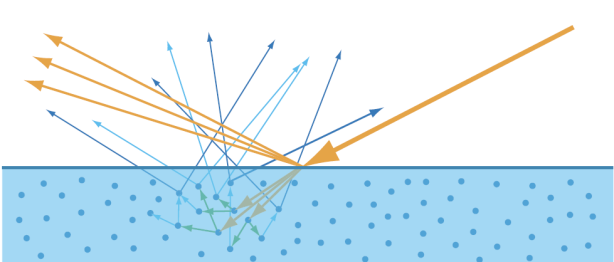
\includegraphics[width=0.7\textwidth]{pics/physicallyBasedRendering/ds} \\
    Specular
    \begin{itemize}
        \item "Zrcadlový" odraz
        \item Dominantní pro kovy
    \end{itemize}
    Diffuse
    \begin{itemize}
        \item Odraz uvnitř materiálu.
        \item Dominantní pro izolanty.
    \end{itemize}
\end{frame}

\begin{frame}
    \frametitle{Cook-Torrance}
    Spekulární odraz
    \begin{equation*}
        f_r(\mathbf x, \mathbf l, \mathbf v) = \frac{F(\mathbf l, \mathbf h)G(\mathbf l, \mathbf v, \mathbf h)D(\mathbf h)}{4(\mathbf n \cdot \mathbf l)(\mathbf n \cdot \mathbf v)}
    \end{equation*}
    \begin{itemize}
        \item F - Fresnell/Schlick
        \item D - Distribuční funkce plošek
        \item G - Geometrické zastínění plošek
    \end{itemize}
\end{frame}

\begin{frame}
    \frametitle{Blinn-Phong}
    \begin{equation*}
        D(\mathbf h) = (\mathbf n \cdot \mathbf h)^{\mathrm shininess}
    \end{equation*}
    \includegraphics[width=.5\textwidth]{pics/physicallyBasedRendering/shininessGraph}
    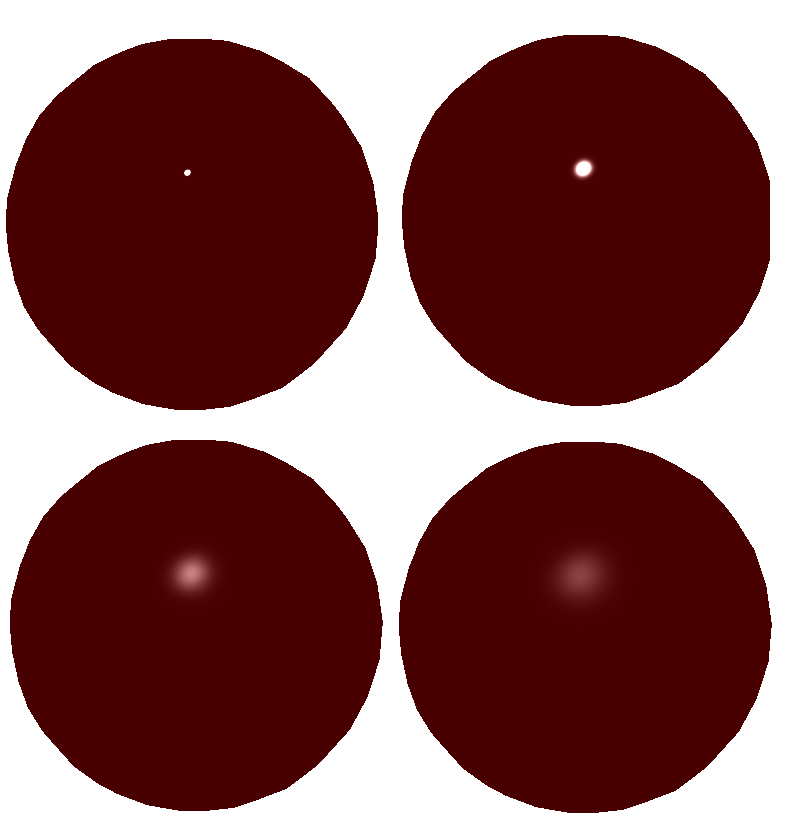
\includegraphics[width=.5\textwidth]{pics/physicallyBasedRendering/shininess.png}
\end{frame}

\begin{frame}
    \frametitle{Dohromady}
    \begin{equation*}
        f_r(\mathbf x, \mathbf l, \mathbf v) = (R_0 + (1-R_0)(1-(\mathbf l \cdot \mathbf h))^5)(\mathbf n \cdot \mathbf h)^{\mathrm shininess}
    \end{equation*}
    Co chybí?
    \begin{itemize}
        \item Barva materiálu (izolantú). $R_0$ je "barva kovu".
        \item[!] Lomené paprsky.
        \item Zachování energie.
    \end{itemize}
\end{frame}

\begin{frame}
    \frametitle{Difúzní odraz}
    \begin{equation*}
        f_r(\mathbf x, \mathbf l, \mathbf v) = \frac{k_d}{\pi}
    \end{equation*}
    \begin{itemize}
        \item Nezáleží na poloze pozorovatele.
        \item $1/\pi$ je zachování energie.
    \end{itemize}
    \begin{equation*}
        \int\limits_\Omega 1/\pi d\omega = 1
    \end{equation*}
\end{frame}

\begin{frame}
    \frametitle{Diffuse + Specular}
    \begin{equation*}
        \left(\frac{k_s}{\pi} + k_n(R_0 + (1-R_0)(1-(\mathbf l \cdot \mathbf h))^5)(\mathbf n \cdot \mathbf h)^{\mathrm shininess}\right)(\mathbf n \cdot \mathbf l)
    \end{equation*}
    \begin{equation*}
        k_n = \frac{(\mathrm shininess + 2)(\mathrm shininess + 4)}{8\pi(2^{-\frac{shininess}{2}} + shininess)}
    \end{equation*}
    \begin{itemize}
        \item $\mathbf n \cdot \mathbf l$ z renderovací rovnice.
        \item Zachování energie pro specular.
        \item Odvození na \url{http://www.farbrausch.de/~fg/stuff/phong.pdf}
    \end{itemize}
\end{frame}

\section{Bodový zdroj světla}

\begin{frame}
    \frametitle{Bodový zdroj světla}
    \begin{equation*}
        L_o(\mathbf x, \omega, \lambda, t) = L_e(\mathbf x, \omega, \lambda, t) + \int\limits_\Omega f_r(\mathbf x, \omega', \omega, \lambda, t) L_i(\mathbf x, \omega', \lambda, t) (-\omega' \cdot \mathbf n) d \omega'
    \end{equation*}
    \begin{itemize}
        \item Bod má nulovou plochu.
        \item Bodové zdroje jsou singularity.
        \item Jak upravit renderovací rovnici? Jaké $L_i$?
        \pause
        \item Nastavíme ho přes barvu ideálního difúzního povrchu.
    \end{itemize}
    \begin{align*}
        L_o &= \int\limits_\Omega \frac{1}{\pi} L_i (-\omega' \cdot \mathbf n) d \omega' \\
        L_i &= \pi L_o
    \end{align*}
\end{frame}

\begin{frame}
    \frametitle{Pohromadě}
    \begin{equation*}
        L = \sum_i \left(\frac{k_s}{\pi} + k_n F(R_0, \mathbf l_i,\mathbf h_i)(\mathbf n \cdot \mathbf h_i)^{\mathrm shininess}\right)(\mathbf n \cdot \mathbf l_i) \pi L_i
    \end{equation*}
    \begin{itemize}
        \item Sčítáme přes světla.
        \item $\pi$ se vykrátí.
    \end{itemize}
    \pause
    \vfill
    Co tam chybí?
    \pause
    \begin{itemize}
        \item Vzdálenost od světla $L_i = f(|\mathbf p_i - \mathbf x|^2)$
        \item Světelný kužel.
        \item Vícenásobný odraz světla.
    \end{itemize}
\end{frame}

\begin{frame}
    \frametitle{Ambientní světlo}
    \begin{align*}
        L_o &= \sum_i k_a L_i \\
        k_a &= k_d 
    \end{align*}
    \vfill
    
\includegraphics[width=2.5in]{pics/physicallyBasedRendering/ambient}
    \begin{itemize}
        \item Hrubá aproximace mnohonásobného odrazu světla.
    \end{itemize}
\end{frame}

\section{Normály}

\begin{frame}
    \frametitle{Normálové vektory}

    \begin{itemize}
        \item Kolmé k povrchu
        \item $\left| N \right| = 1$ (normalizované)
        \item 1 na trojúhelník/1 na vrchol
        \vfill
        \item $\displaystyle \vec{N_{\mathrm{face}}} = \vec{AB} \times \vec{AC}$
        \item $\displaystyle \vec{N_{\mathrm{vertex}}} = \mathrm{normalize}\left( \sum\limits_{i=1}^n N_{\mathrm{face}i} \right)$
        \item Prúměr vážený plochou trojúhelníkú
        \vfill
        \item Transformace :
        \begin{itemize}
            \item Rotace \emph{+ posun} - $N_{\mathrm{eye}} = ModelView \cdot N_{\mathrm{model}}$
            \item Scale - $N_{\mathrm{eye}} = (ModelView^T)^{-1} \cdot N_{\mathrm{model}}$
            \item[\color{red}!] Při scale je nutné vektory po transformaci znovu normalizovat!
        \end{itemize}
    \end{itemize}
\end{frame}

\begin{frame}
    \frametitle{Stínování}

    "Flat" stínování
    \begin{itemize}
        \item Osvětlují se celé trojúhelníky.
        \item Nic se neinterpoluje.
    \end{itemize}

    Gouraudovo stínování - "per vertex lighting"
    \begin{itemize}
        \item Osvětlení se počítá pro vrcholy.
        \item Interpolují se barvy.
        \item Dnes už nemá smysl.
    \end{itemize}

    Phongovo stínování - "per fragment lighting"
    \begin{itemize}
        \item Osvětlení se počítá pro fragmenty.
        \item Interpolují se normálové vektory.
    \end{itemize}

    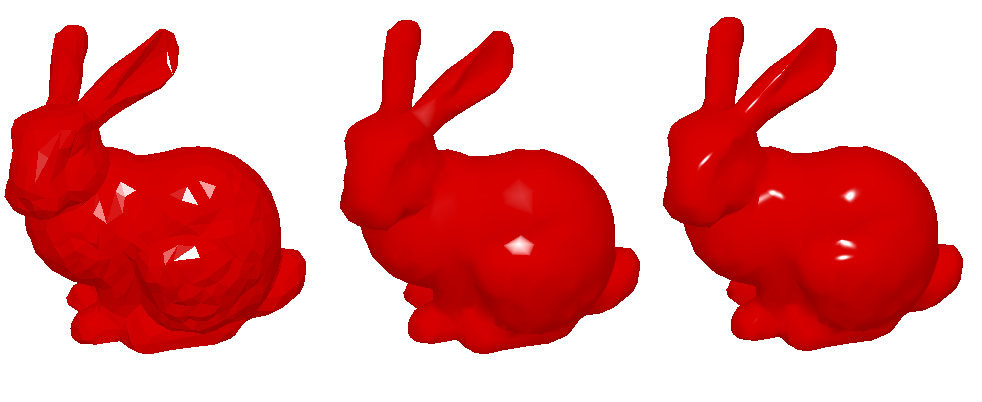
\includegraphics[width=\textwidth]{pics/physicallyBasedRendering/shading}
\end{frame}


\setbeamercolor{background canvas}{bg=fitblue}
\begin{frame}
\frametitle{Textury}
\begin{center}
\Huge {\color{white}Textury}
\end{center}
\end{frame}
\setbeamercolor{background canvas}{bg=white}

\begin{frame}[fragile]
\frametitle{Textury - nahrání rastrových dat}
	\begin{itemize}
	\item Textura je rastrový obrázek, který se namapuje na geometrii.
	\item V OpenGL je to objekt.
\end{itemize}
{\scriptsize
\begin{minted}[bgcolor=bg]{packages/c_cpp.py:CppLexer -x}
//vytvoreni jmena textury
glCreateTextures(GL_TEXTURE_2D,1,&tColor);//vygenerovani jmeno textury pro barvu

//nastaveni parametru textury
//filtering
glTextureParameteri(tColor,GL_TEXTURE_MAG_FILTER,GL_NEAREST);
glTextureParameteri(tColor,GL_TEXTURE_MIN_FILTER,GL_NEAREST);

//wrapping
glTextureParameteri(tColor,GL_TEXTURE_WRAP_S,GL_CLAMP_TO_EDGE);
glTextureParameteri(tColor,GL_TEXTURE_WRAP_T,GL_REPEAT);

//alokace a nahrani dat na GPU
glTextureImage2DEXT(tColor,GL_TEXTURE_2D,0,//alokujeme misto
  GL_RGBA32F,//format ulozeni na GPU (4*float pro pixel)
  WIDTH,HEIGHT,0,GL_RGBA,//format ulozeni dan na CPU
  GL_UNSIGNED_BYTE,//typ dat na CPU
  Data);//data na CPU
\end{minted}
}
\end{frame}

\begin{frame}[fragile]
\frametitle{Nastavení textur}
	\begin{itemize}
	\item V Shader Programu se k nim přistupuje přes uniformní proměnné.
	\item Textura se naváže k texturovací jednotce.
	\item Uniformní proměnná se naváže na texturovací jednotku.
	\end{itemize}
	\begin{figure}[h]
		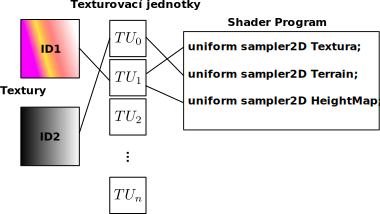
\includegraphics[width=10cm,keepaspectratio]{pics/texture/tu.pdf}
	\end{figure}
\end{frame}

\begin{frame}[fragile]
\frametitle{Nastavení textur}
Shader Program:
{\scriptsize
\begin{minted}[bgcolor=bg]{packages/graphics.py:GLShaderLexer -x}
#version 330
layout(binding=0)uniform sampler2D Textura;
layout(binding=1)uniform sampler2D Terrain;
layout(binding=1)uniform sampler2D HeightMap;
void main(){
  texture(Texture,coords);
  //...
\end{minted}
}
Aplikace:
{\scriptsize
\begin{minted}[bgcolor=bg]{packages/c_cpp.py:CppLexer -x}
//pripojemni textur k texurovacim jednotkam
glBindTextureUnit(0,ID2);
glBindTextureUnit(1,ID1);
\end{minted}
}
\end{frame}

\begin{frame}[fragile]
\frametitle{Adresování textur}
	\begin{itemize}
	\item Textura se adresuje texturovacími koordináty.
	\item Velikost Textury nehraje roli.
	\item Levý dolní roh 2D textury má souřadnice (0.0f,0.0f)
	\item Pravý horní roh 2D textury má souřadnice (1.0f,1.0f)
	\end{itemize}
	\begin{figure}[h]
		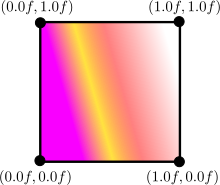
\includegraphics[width=5cm,keepaspectratio]{pics/texture/textura.pdf}
	\end{figure}
\end{frame}

\begin{frame}[fragile]
\frametitle{Atlas textur}
	\begin{itemize}
	\item Více obrázků v jedné textuře.
	\item Staří jedna texturovací jednotka.
	\item Zamezíme přepínání.
	\end{itemize}
	\begin{figure}[h]
		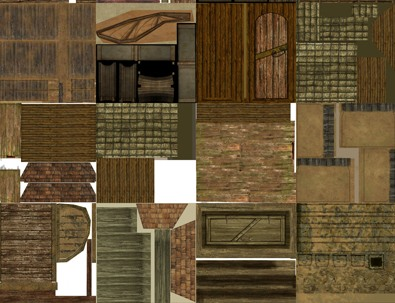
\includegraphics[width=5cm,keepaspectratio]{pics/texture/textureatlas.jpg}
	\end{figure}
	\url{http://www.scriptspot.com/3ds-max/scripts/texture-atlas-generator}
\end{frame}


\setbeamercolor{background canvas}{bg=fitblue}
\begin{frame}
\frametitle{Framebuffer}
\begin{center}
\Huge {\color{white}Framebuffer}
\end{center}
\end{frame}
\setbeamercolor{background canvas}{bg=white}

\begin{frame}[fragile]
\frametitle{Frame Buffer Object (FBO)}
  \begin{itemize}
    \item Obvykle se scéna renderuje do defaultního framebufferu obrazovky.
    \item Od verze OpenGL 3.3 je umožněno vytvoření vlastního framebufferu a vykreslovat scénu do něj.
    \item Framebuffer se skládá z několika 2D polí (hloubkový buffer, stencil buffer, několik barevných bufferů).
    \item{FBO umožňují renderování do textur.}
    \item{Umožňují renderovat uživatelské informace (normály, pozici, hloubku, ...) (Multiple Render Targets).}
    \item{Jsou základem pro různé grafické efekty např. vody, SSAO.}
    \item{Umožňují odložené stínování (deferred shading).}
    \item{Layered rendering}
  \end{itemize}
\end{frame}

\begin{frame}
\frametitle{Frame Buffer Object}
  \begin{figure}[h]
  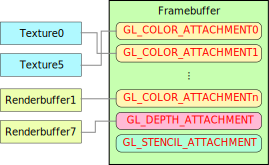
\includegraphics[width=10cm,keepaspectratio]{pics/framebuffer/framebuffer.pdf}
  \end{figure}
\end{frame}


\begin{frame}
\frametitle{Použití FBO}
    \begin{enumerate}
        \item{Získání jména FBO.}
        \item{Aktivování FBO.}
        \item{Připojení textur/renderbufferů k attachmentům.}
        \item{Nastavení seznamu attachmentů.}
        \item{Deaktivace FBO.}
        \item{...}
        \item{Aktivování FBO.}
        \item{Vykreslení scény.}
        \item{Deaktivace FBO.}
        \item{Zpracování vyrenderovaných textur.}
    \end{enumerate}
\end{frame}

\begin{frame}[fragile]
\frametitle{Vytvoření/uvolnění FBO identifikátorů}
  \begin{itemize}
    \item{
    Vytvoření VBO identifikátorů:
{\scriptsize
\begin{minted}[bgcolor=bg]{packages/c_cpp.py:CppLexer -x}
void glCreateFramebuffers(GLsizei n,GLuint * buffers);
\end{minted}
}}
    \item{
    Uvolnění VBO identifikátorů:
{\scriptsize
\begin{minted}[bgcolor=bg]{packages/c_cpp.py:CppLexer -x}
void glDeleteFramebuffers(GLsizei n,GLuint * buffers);
\end{minted}
}}
  \end{itemize}
\end{frame}

\begin{frame}[fragile]
\frametitle{Ověření stavu FBO}
  \begin{itemize}
    \item{
    Pro ověření stavu FBO použijeme tuto funkci
{\scriptsize
\begin{minted}[bgcolor=bg]{packages/c_cpp.py:CppLexer -x}
GLenum glCheckNamedFramebufferStatus(GLuint fbo,GLenum target);
\end{minted}
}}
    \item{
    Pokud funkce vraci {\color{red} GL\_FRAMEBUFFER\_COMPLETE} je vše v pořádku.
    }
  \end{itemize}
\end{frame}


\begin{frame}[fragile]
\frametitle{Aktivování/deaktivování FBO}
  \begin{itemize}
    \item{
    Aktivování/deaktivování FBO:
{\scriptsize
\begin{minted}[bgcolor=bg]{packages/c_cpp.py:CppLexer -x}
void glBindFramebuffer(GLenum target,GLuint framebuffer);
\end{minted}
}
    \begin{description}
    \item[target] GL\_FRAMEBUFFER stejný buffer pro čtení i zápis, GL\_READ\_FRAMEBUFFER, GL\_DRAW\_FRAMEBUFFER.
    \item[framebuffer] Jméno FBO získané {\color{blue} glCreateFramebuffers}.
    Pokud nastaveno na 0 deaktivuje buffer.
    \end{description}
    }
  \end{itemize}
\end{frame}

\begin{frame}[fragile]
\frametitle{Připojení textur}
  \begin{itemize}
    \item{
    Attachment představuje jeden podbuffer FBO - například hloubkový buffer.
    Připojení textur k attachmentům:
{\scriptsize
\begin{minted}[bgcolor=bg]{packages/c_cpp.py:CppLexer -x}
void glNamedFramebufferTexture(GLuint fbo,GLenum attachment,
  GLuint texture,GLint level);
\end{minted}
}
    \begin{description}
    \item[fbo] framebuffer
    \item[attachment] Které informace budeme zapisovat do textury.
    GL\_DEPTH\_ATTACHMENT - hloubkový buffer.
    GL\_STENCIL\_ATTACHMENT - stencil buffer.
    GL\_COLOR\_BUFFERx - barva, nebo jiná informace.
    Specifikováno pomocí fragment shaderu (layout).
    \item[texture] Identifikátor textury.
    \item[level] Stupeň mipmappingu.
    \end{description}
    }
    \item Layered rendering
{\scriptsize
\begin{minted}[bgcolor=bg]{packages/c_cpp.py:CppLexer -x}
void glNamedFramebufferTextureLayer(GLuint fbo,GLenum attachment,
  GLuint texture,GLint level,GLint layer);
\end{minted}
}
  \end{itemize}
\end{frame}

\begin{frame}[fragile]
\frametitle{Nastavení seznamu attachmentů (MRT)}
  \begin{itemize}
    \item{
    Nastavením seznamu attachmentů definujeme, do kterých barevných bufferů se bude kreslit.
{\scriptsize
\begin{minted}[bgcolor=bg]{packages/c_cpp.py:CppLexer -x}
void glNamedFramebufferDrawBuffers(GLuint id,GLsizei n,const GLenum * bufs);
\end{minted}
}
    \begin{description}
    \item[id] framebuffer
    \item[n] Počet bufferů, do kterých budeme kreslit.
    \item[bufs] Seznam GL\_COLOR\_BUFFERx.
    Pořadí specifikuje, ke kterému layout ve fragment shaderu bude buffer navázán.
    \end{description}
    }
  \end{itemize}
\end{frame}

\begin{frame}[fragile]
\frametitle{Kompletní příklad}
    Do textur budeme vykreslovat barvu, normálu a hloubku.
    Fragment shader:
{\scriptsize
\begin{minted}[bgcolor=bg]{packages/graphics.py:GLShaderLexer -x}
#version 430
layout(location=0)out vec4 fragColor;//jeden vystup - drawbuffer0
layout(location=1)out vec3 fragNormal;//druhy vystup - drawbuffer1
//...
void main(){
  //...
  fragColor=vec4(fCol,1);//zapis barvy
  fragNormal=(fNor+1)/2;//zapis normaly
}
\end{minted}
}
\end{frame}

\begin{frame}[fragile]
\frametitle{Kompletní příklad}
    Aplikace - inicializace:
    {\tiny
\begin{minted}[bgcolor=bg]{packages/c_cpp.py:CppLexer -x}
glTexImage2D(GL_TEXTURE_2D,0,GL_RGBA8F,WIDTH,HEIGHT,0,GL_RGBA,
  GL_UNSIGNED_BYTE,NULL);//alokujeme misto
//...
glTexImage2D(GL_TEXTURE_2D,0,GL_RGB32F,WIDTH,HEIGHT,0,GL_RGBA,
  GL_UNSIGNED_BYTE,NULL);//alokujeme misto
//...
glTexImage2D(GL_TEXTURE_2D,0,GL_DEPTH_COMPONENT24,
  WIDTH,HEIGHT,0,GL_DEPTH_COMPONENT,GL_UNSIGNED_BYTE,NULL);

glCreateFramebuffers(1,&fbo);//vygenerujeme nazev pro FBO

//navazani textur
glNamedFramebufferTexture(fbo,GL_DEPTH_ATTACHMENT,
  tDepth,0);//navazeme texturu pro hloubku
glNamedFramebufferTexture(fbo,GL_COLOR_ATTACHMENT3,
  tColor,0);//navazeme texturu pro barvu
glNamedFramebufferTexture(GL_FRAMEBUFFER,GL_COLOR_ATTACHMENT5,
  tNormal,0);//navazeme texturu pro normalu

GLenum drawBuffers[]={
  GL_COLOR_ATTACHMENT3,//layout(location=0)out vec4 fragColor;
  GL_COLOR_ATTACHMENT5//layout(location=1)out vec3 fragNormal;
};
glNamedFramebufferDrawBuffers(fbo,2,drawBuffers);//nastavime seznam cilu

if(glCheckNamedFramebufferStatus(fbo,GL_FRAMEBUFFER)!=GL_FRAMEBUFFER_COMPLETE)
  std::cerr<<"chyba\n";
glBindFramebuffer(GL_FRAMEBUFFER,0);
    \end{minted}
    }
\end{frame}

\begin{frame}[fragile]
\frametitle{Kompletní příklad}
    Aplikace - kresleni:
{\scriptsize
\begin{minted}[bgcolor=bg]{packages/c_cpp.py:CppLexer -x}
glBindFramebuffer(GL_FRAMEBUFFER,FBO);//aktivujeme FBO
glDrawArrays(...);
glBindFramebuffer(GL_FRAMEBUFFER,0);//deaktivovani FBO
\end{minted}
}
\end{frame}

\setbeamercolor{background canvas}{bg=fitblue}
\begin{frame}
\frametitle{Hierarchický depth buffer}
\begin{center}
\Huge {\color{white}Hierarchický depth buffer}
\end{center}
\end{frame}
\setbeamercolor{background canvas}{bg=white}

\begin{frame}[fragile]
\frametitle{Kompletní příklad tvorba hier. z-bufferu}
		GLSL - CreateHierarchy:
{\tiny
\begin{minted}[bgcolor=bg]{packages/graphics.py:GLShaderLexer -x}
//vertex shader////////////////////////////////////////////////////////////
#version 430
void main(){
  gl_Position=vec4(0);
}
//geometry shader//////////////////////////////////////////////////////////
#version 430
layout(points)in;
layout(triangle_strip,max_vertices=4)out;
void main(){
  gl_Position=vec4(-1,-1,0,1);EmitVertex();
  gl_Position=vec4(+1,-1,0,1);EmitVertex();
  gl_Position=vec4(-1,+1,0,1);EmitVertex();
  gl_Position=vec4(+1,+1,0,1);EmitVertex();
}
//fragment shader///////////////////////////////////////////////////////////
#version 430
layout(binding=0)uniform sampler2D Last;//last mipmap
layout(location=0)out vec2 fDepth;//output depth
ivec2 Coord=ivec2(gl_FragCoord.xy);//coordinates
void main(void){
  vec2 A=texelFetch(Last,Coord*2+ivec2(0,0),0).xy;
  vec2 B=texelFetch(Last,Coord*2+ivec2(1,0),0).xy;
  vec2 C=texelFetch(Last,Coord*2+ivec2(0,1),0).xy;
  vec2 D=texelFetch(Last,Coord*2+ivec2(1,1),0).xy;
  fDepth=vec2(min(min(A.x,B.x),min(C.x,D.x)),max(max(A.y,B.y),max(C.y,D.y)));
}
		\end{minted}
		}
\end{frame}

\begin{frame}[fragile]
\frametitle{Kompletní příklad tvorba hier. z-bufferu}
		Aplikace - inicializace:
{\scriptsize
\begin{minted}[bgcolor=bg]{packages/c_cpp.py:CppLexer -x}
glCreateTextures(GL_TEXTURE_2D,1,&Depth);
//textura obsahujici minimalni a maximalni hloubku
glBindTexture(GL_TEXTURE_2D,Depth);
glTextureParameteri(Depth,GL_TEXTURE_MAG_FILTER,GL_NEAREST);
glTextureParameteri(Depth,GL_TEXTURE_MIN_FILTER,GL_NEAREST_MIPMAP_NEAREST);
int Size=WSize;
int Level=0;
while(Size>0){//smycka pres levely
  glTextureImage2DEXT(Depth,GL_TEXTURE_2D,Level++,GL_RG32F,Size,Size,0,GL_RG,
    GL_FLOAT,NULL);//alokace vrstvy
  Size/=2;
}
//render buffer s hloubkou
glCreateRenderbuffers(1,&RBO_Depth);
glNamedRenderbufferStorage(RBO_Depth,GL_DEPTH_COMPONENT,WSize,WSize);

glCreateFramebuffers(1,&FBO);//vygenerujeme nazev pro FBO
		\end{minted}
		}
\end{frame}


\begin{frame}[fragile]
\frametitle{Kompletní příklad tvorba hier. z-bufferu}
		Aplikace - render2 - tvorba hierarchie:
{\scriptsize
\begin{minted}[bgcolor=bg]{packages/c_cpp.py:CppLexer -x}
glUseProgram(CreateHierarchy);
int Level=1;
int ActSize=WSize/2;
glBindFramebuffer(GL_FRAMEBUFFER,HFBO);//bind framebuffer
glBindTextureUnit(0,Depth);//bind depth texture to tex. unit 0
while(ActSize>0){//while there are
  glViewport(0,0,ActSize,ActSize);//set viewport
  glTextureParameteri(Depth,GL_TEXTURE_BASE_LEVEL,Level-1);//starting mipmap level
  glTextureParameteri(Depth,GL_TEXTURE_MAX_LEVEL,Level-1);//max mipmap level
  glNamedFramebufferTexture(FBO,GL_COLOR_ATTACHMENT0,Depth,Level);
  GLenum DrawBuffers[]={GL_COLOR_ATTACHMENT0};
  glNamedFramebufferDrawBuffers(1,DrawBuffers);
  glDrawArrays(GL_POINTS,0,1);
  Level++;//increment level of mipmap
  ActSize/=2;//actual size of mipmap
}
glBindFramebuffer(GL_FRAMEBUFFER,0);//unbind framebffer
glTextureParameteri(Depth, GL_TEXTURE_BASE_LEVEL, 0);//starting mipmap level
glTextureParameteri(Depth, GL_TEXTURE_MAX_LEVEL, Level-1);//max mipmap level
glViewport(0,0,WSize,WSize);//reset viewport
\end{minted}
}
\end{frame}


\setbeamercolor{background canvas}{bg=fitblue}
\begin{frame}
\frametitle{Layered Rendering}
\begin{center}
\Huge {\color{white}Layered Rendering}
\end{center}
\end{frame}
\setbeamercolor{background canvas}{bg=white}

\begin{frame}[fragile]
\frametitle{Layered rendering, cube map}
Cube map rendering - CPU
{\scriptsize
\begin{minted}[bgcolor=bg]{packages/c_cpp.py:CppLexer -x}
GLuint cubeMap;
glCreateTextures(GL_TEXTURE_CUBE_MAP,1,&cubeMap);
for(size_t i=0;i<6;++i)
  glTextureImage2DEXT(cubeMap,GL_TEXTURE_CUBE_MAP_POSITIVE_X+i,0,
    GL_RGBA8,width,height,0,GL_RGBA,GL_UNSIGNED_BYTE,nullptr);
//it will attach all six sides of cube map
glNamedFramebufferTexture(cubeMap,GL_COLOR_ATTACHMENT0,cubeMap,0);
\end{minted}
}
\end{frame}

\begin{frame}[fragile]
\frametitle{Layered rendering, cube map}
Cube map rendering - Vertex Shader
{\scriptsize
\begin{minted}[bgcolor=bg]{packages/graphics.py:GLShaderLexer -x}
layout(location=0)in vec3 position;
uniform float near = 0.1;
uniform float far  = 1000;
uniform vec4 lightPosition = vec4(0,0,0,1);
out int vInstanceID;
void main(){
  const mat4 views[6] = {
    mat4(vec4(+0,+0,-1,0), vec4(+0,-1,+0,0), vec4(-1,+0,+0,0), vec4(0,0,0,1)),
    mat4(vec4(+0,+0,+1,0), vec4(+0,-1,+0,0), vec4(+1,+0,+0,0), vec4(0,0,0,1)),
    mat4(vec4(+1,+0,+0,0), vec4(+0,+0,-1,0), vec4(+0,+1,+0,0), vec4(0,0,0,1)),
    mat4(vec4(+1,+0,+0,0), vec4(+0,+0,+1,0), vec4(+0,-1,+0,0), vec4(0,0,0,1)),
    mat4(vec4(+1,+0,+0,0), vec4(+0,-1,+0,0), vec4(+0,+0,-1,0), vec4(0,0,0,1)),
    mat4(vec4(-1,+0,+0,0), vec4(+0,-1,+0,0), vec4(+0,+0,+1,0), vec4(0,0,0,1))
  };

  mat4 projection = mat4(
    vec4(1,0,0,0),
    vec4(0,1,0,0),
    vec4(0,0,-(far+near)/(far-near),-1),
    vec4(0,0,-2*far*near/(far-near),0));
  gl_Position = projection*views[gl_InstanceID]*vec4(position-lightPosition.xyz,1);
  vInstanceID = gl_InstanceID;
}
\end{minted}
}
\end{frame}


\begin{frame}[fragile]
\frametitle{Layered rendering, cube map}
Cube map rendering - Geometry shader
{\scriptsize
\begin{minted}[bgcolor=bg]{packages/graphics.py:GLShaderLexer -x}
layout(triangles)in;
layout(triangle_strip,max_vertices=3)out;
in int vInstanceID[];
void main(){
  gl_Layer = vInstanceID[0];
  gl_Position = gl_in[0].gl_Position;EmitVertex();
  gl_Position = gl_in[1].gl_Position;EmitVertex();
  gl_Position = gl_in[2].gl_Position;EmitVertex();
  EndPrimitive();
}
\end{minted}
}
\end{frame}



%\input{src/transformFeedback}
%\input{src/tessellation}
%\begin{frame}
\frametitle{Beziérová křivka}
$$
{\color{magenta}\vec{P}_{0,1,2,3}(t)}=(1,t^1,t^2,t^3)\cdot
\left(
\begin{array}{cccc}
 1 &  0 &  0 &  0 \\
-3 &  3 &  0 &  0 \\
 3 & -6 &  3 &  0 \\
-1 &  3 & -3 &  1
\end{array}
\right)
\cdot
\left(
\begin{array}{c}
  {\color{green}\vec{P}_{0}} \\
  {\color{green}\vec{P}_{1}} \\
  {\color{green}\vec{P}_{2}} \\
  {\color{green}\vec{P}_{3}} 
\end{array}
\right)
$$
\end{frame}


\begin{frame}
\frametitle{Beziérová křivka}
  \begin{figure}[h]
  \includegraphics[width=8cm,keepaspectratio]{pics/bezier/bezier}
  \end{figure}
  {\scriptsize
  \[
  \begin{array}{lclcl}
    \color{red}    {\vec{P}_{0,1}    } &=& (1-t)\color{green}{\vec{P}_0      } &+& (t)\color{green}{\vec{P}_1      } \\
    \color{red}    {\vec{P}_{1,2}    } &=& (1-t)\color{green}{\vec{P}_1      } &+& (t)\color{green}{\vec{P}_2      } \\
    \color{red}    {\vec{P}_{2,3}    } &=& (1-t)\color{green}{\vec{P}_2      } &+& (t)\color{green}{\vec{P}_3      } \\
    \color{blue}   {\vec{P}_{0,1,2}  } &=& (1-t)\color{red}  {\vec{P}_{0,1}  } &+& (t)\color{red}  {\vec{P}_{1,2}  } \\
    \color{blue}   {\vec{P}_{1,2,3}  } &=& (1-t)\color{red}  {\vec{P}_{1,2}  } &+& (t)\color{red}  {\vec{P}_{2,3}  } \\
    \color{magenta}{\vec{P}_{0,1,2,3}} &=& (1-t)\color{blue} {\vec{P}_{0,1,2}} &+& (t)\color{blue} {\vec{P}_{1,2,3}} 
  \end{array}
  \]
  }
\end{frame}

\begin{frame}
\frametitle{Beziérová křivka}
  {\tiny
  \[
  \begin{array}{lclcl}
    \color{red}    {\vec{P}_{0,1}    } &=& (1-t)\color{green}{\vec{P}_0      } &+& (t)\color{green}{\vec{P}_1      } \\
    \color{red}    {\vec{P}_{1,2}    } &=& (1-t)\color{green}{\vec{P}_1      } &+& (t)\color{green}{\vec{P}_2      } \\
    \color{red}    {\vec{P}_{2,3}    } &=& (1-t)\color{green}{\vec{P}_2      } &+& (t)\color{green}{\vec{P}_3      } \\
    \color{blue}   {\vec{P}_{0,1,2}  } &=& (1-t)\color{red}  {\vec{P}_{0,1}  } &+& (t)\color{red}  {\vec{P}_{1,2}  } \\
    \color{blue}   {\vec{P}_{1,2,3}  } &=& (1-t)\color{red}  {\vec{P}_{1,2}  } &+& (t)\color{red}  {\vec{P}_{2,3}  } \\
    \color{magenta}{\vec{P}_{0,1,2,3}} &=& (1-t)\color{blue} {\vec{P}_{0,1,2}} &+& (t)\color{blue} {\vec{P}_{1,2,3}} 
  \end{array}
  \]
  }
  {\tiny
  \[
  \begin{array}{lclcl}
    \color{blue}   {\vec{P}_{0,1,2}  } &=& (1-t)((1-t){\color{green}\vec{P}_0} + (t){\color{green}\vec{P}_1}) &+& (t)((1-t){\color{green}\vec{P}_1} + (t){\color{green}\vec{P}_2}) \\
    \color{blue}   {\vec{P}_{1,2,3}  } &=& (1-t)((1-t){\color{green}\vec{P}_1} + (t){\color{green}\vec{P}_2}) &+& (t)((1-t){\color{green}\vec{P}_2} + (t){\color{green}\vec{P}_3}) \\
    \color{magenta}{\vec{P}_{0,1,2,3}} &=& (1-t)\color{blue} {\vec{P}_{0,1,2}} &+& (t)\color{blue} {\vec{P}_{1,2,3}} 
  \end{array}
  \]
  }
  {\tiny
  \[
  \begin{array}{lclccrc}
    \color{magenta}{\vec{P}_{0,1,2,3}} &=& (1-t)&(1-t)&(1-t)&{\color{green}\vec{P}_0} &+ \\
                                       & & (1-t)&(1-t)&(  t)&{\color{green}\vec{P}_1} &+ \\
                                       & & (1-t)&(  t)&(1-t)&{\color{green}\vec{P}_1} &+ \\
                                       & & (1-t)&(  t)&(  t)&{\color{green}\vec{P}_2} &+ \\
                                       & & (  t)&(1-t)&(1-t)&{\color{green}\vec{P}_1} &+ \\
                                       & & (  t)&(1-t)&(  t)&{\color{green}\vec{P}_2} &+ \\
                                       & & (  t)&(  t)&(1-t)&{\color{green}\vec{P}_2} &+ \\
                                       & & (  t)&(  t)&(  t)&{\color{green}\vec{P}_3} &
  \end{array}
  \]
  }
  {\tiny
  \[
  \begin{array}{lclccrc}
    \color{magenta}{\vec{P}_{0,1,2,3}} &=& (1-t)&(1-t)&(1-t)&{\color{green}\vec{P}_0} &+ \\
                                       & & 3(1-t)&(1-t)&(  t)&{\color{green}\vec{P}_1} &+ \\
                                       & & 3(1-t)&(  t)&(  t)&{\color{green}\vec{P}_2} &+ \\
                                       & & (  t)&(  t)&(  t)&{\color{green}\vec{P}_3} &
  \end{array}
  \]
  }

\end{frame}

\begin{frame}
\frametitle{Beziérová křivka}
  {\tiny
  \[
  \begin{array}{lclccrc}
    \color{magenta}{\vec{P}_{0,1,2,3}} &=& (1-t)&(1-t)&(1-t)&{\color{green}\vec{P}_0} &+ \\
                                       & & 3(1-t)&(1-t)&(  t)&{\color{green}\vec{P}_1} &+ \\
                                       & & 3(1-t)&(  t)&(  t)&{\color{green}\vec{P}_2} &+ \\
                                       & & (  t)&(  t)&(  t)&{\color{green}\vec{P}_3} &
  \end{array}
  \]
  }
  {\tiny
  \[
  \begin{array}{lclrc}
    \color{magenta}{\vec{P}_{0,1,2,3}} &=& (1-t)^3&{\color{green}\vec{P}_0} &+ \\
                                       & & 3(1-t)^2(t)&{\color{green}\vec{P}_1} &+ \\
                                       & & 3(1-t)(t)^2&{\color{green}\vec{P}_2} &+ \\
                                       & & (t)^3&{\color{green}\vec{P}_3} &
  \end{array}
  \]
  }
  {\tiny
  \[
  \begin{array}{lclrc}
    \color{magenta}{\vec{P}_{0,1,2,3}} &=& \dbinom{3}{0}(1-t)^{3-0}(t)^{0}&{\color{green}\vec{P}_0} &+ \\
                                       & & \dbinom{3}{1}(1-t)^{3-1}(t)^{1}&{\color{green}\vec{P}_1} &+ \\
                                       & & \dbinom{3}{2}(1-t)^{3-2}(t)^{2}&{\color{green}\vec{P}_2} &+ \\
                                       & & \dbinom{3}{3}(1-t)^{3-3}(t)^{3}&{\color{green}\vec{P}_3} &
  \end{array}
  \]
  }
  {\tiny
  $$
  {\color{magenta}\vec{P}_{0,1,2,3}(t)} = \sum\limits_{i=0}^{i \leq 3}\dbinom{3}{i}(1-t)^{3-i}(t)^{i}{\color{green}\vec{P}_i} 
  $$
  }
  {\tiny
  $$
  {\color{magenta}\vec{P}(t)} = \sum\limits_{i=0}^{i \leq n-1}\dbinom{n-1}{i}(1-t)^{n-1-i}(t)^{i}{\color{green}\vec{P}_i} 
  $$
  }


\end{frame}

\begin{frame}
\frametitle{Beziérová křivka}
  {\tiny
  \[
  \begin{array}{lclrc}
    \color{magenta}{\vec{P}_{0,1,2,3}(t)} &=& (1-t)^3&{\color{green}\vec{P}_0} &+ \\
                                       & & 3(1-t)^2(t)&{\color{green}\vec{P}_1} &+ \\
                                       & & 3(1-t)(t)^2&{\color{green}\vec{P}_2} &+ \\
                                       & & (t)^3&{\color{green}\vec{P}_3} &
  \end{array}
  \]
  }
  {\tiny
  \[
  \begin{array}{lclrc}
    \color{magenta}{\vec{P}_{0,1,2,3}(t)} &=& (1-3t+3t^2-t^3)&{\color{green}\vec{P}_0} &+ \\
                                       & & (3t-6t^2+3t^3)&{\color{green}\vec{P}_1} &+ \\
                                       & & (3t^2-3t^3)&{\color{green}\vec{P}_2} &+ \\
                                       & & (t^3)&{\color{green}\vec{P}_3} &
  \end{array}
  \]
  }
  {\tiny
$$
{\color{magenta}\vec{P}_{0,1,2,3}(t)}=(1,t^1,t^2,t^3)\cdot
\left(
\begin{array}{cccc}
 1 &  0 &  0 &  0 \\
-3 &  3 &  0 &  0 \\
 3 & -6 &  3 &  0 \\
-1 &  3 & -3 &  1
\end{array}
\right)
\cdot
\left(
\begin{array}{c}
  {\color{green}\vec{P}_{0}} \\
  {\color{green}\vec{P}_{1}} \\
  {\color{green}\vec{P}_{2}} \\
  {\color{green}\vec{P}_{3}} 
\end{array}
\right)
$$
  }
\end{frame}

\begin{frame}
\frametitle{Beziérová plocha}
  \begin{figure}[h]
  \includegraphics[width=5cm,keepaspectratio]{pics/bezier/bezier3}
  \end{figure}
  {\tiny
  \[
  \begin{array}{ccclllllll}
    {\color{blue}R_{0,0}} &=& (1-l)(1-t){\color{red}Q_{0,0}} &+& (1-l)(t){\color{red}Q_{1,0}}   &+& (l)(1-t){\color{red}Q_{0,1}}   &+& (l)(t){\color{red}Q_{1,1}} \\
    {\color{blue}R_{1,0}} &=& (1-l)(1-t){\color{red}Q_{1,0}} &+& (1-l)(t){\color{red}Q_{2,0}}   &+& (l)(1-t){\color{red}Q_{1,1}}   &+& (l)(t){\color{red}Q_{2,1}} \\
    {\color{blue}R_{2,0}} &=& (1-l)(1-t){\color{red}Q_{2,0}} &+& (1-l)(t){\color{red}Q_{3,0}}   &+& (l)(1-t){\color{red}Q_{2,1}}   &+& (l)(t){\color{red}Q_{3,1}} \\
                         &&&&\vdots &&&& \\
    {\color{blue}R_{i,k}} &=& (1-l)(1-t){\color{red}Q_{i,k}} &+& (1-l)(t){\color{red}Q_{i+1,k}} &+& (l)(1-t){\color{red}Q_{i,k+1}} &+& (l)(t){\color{red}Q_{i+1,k+1}} \\
  \end{array}
  \]
  }
  {\tiny
  \[
  \begin{array}{ccclllllll}
    {\color{blue}R_{i,k}} &=& (1-l)(1-t){\color{red}Q_{i,k}} &+& (1-l)(t){\color{red}Q_{i+1,k}} &+& (l)(1-t){\color{red}Q_{i,k+1}} &+& (l)(t){\color{red}Q_{i+1,k+1}}        \\
    {\color{magenta}S_{i,k}} &=& (1-l)(1-t){\color{blue}R_{i,k}} &+& (1-l)(t){\color{blue}R_{i+1,k}} &+& (l)(1-t){\color{blue}R_{i,k+1}} &+& (l)(t){\color{blue}R_{i+1,k+1}} \\
    {\color{cyan}X_{i,k}} &=& (1-l)(1-t){\color{magenta}S_{i,k}} &+& (1-l)(t){\color{magenta}S_{i+1,k}} &+& (l)(1-t){\color{magenta}S_{i,k+1}} &+& (l)(t){\color{magenta}S_{i+1,k+1}}
  \end{array}
  \]
  }
\end{frame}



%\begin{frame}
\frametitle{Catmullrom}
  \begin{figure}[h]
  \includegraphics[width=5cm,keepaspectratio]{pics/catmullrom/catmullrom}
  \end{figure}
  {\scriptsize
    $$
v(t)=(1,t^1,t^2,t^3)\cdot
\frac{1}{2}\cdot
\left(
\begin{array}{cccc}
 0 &  2 &  0 &  0 \\
-1 &  0 &  1 &  0 \\
 2 & -5 &  4 & -1 \\
-1 &  3 & -3 &  1
\end{array}
\right)
\cdot
\left(
\begin{array}{c}
  {\color{green}P_{0}} \\
  {\color{green}P_{1}} \\
  {\color{green}P_{2}} \\
  {\color{green}P_{3}} 
\end{array}
\right)
$$
  }
\end{frame}

\begin{frame}
\frametitle{Catmullrom}
  \begin{figure}[h]
  \includegraphics[width=5cm,keepaspectratio]{pics/catmullrom/catmullrom2}
  \end{figure}
  {\scriptsize
    \[
    \begin{array}{ccc}
      f(0) &=& {\color{green}P_1} \\
      f(1) &=& {\color{green}P_2} \\
     f'(0) &=& \frac{{\color{green}P_2}-{\color{green}P_0}}{2} \\
     f'(1) &=& \frac{{\color{green}P_3}-{\color{green}P_1}}{2} \\
      f(t) &=& \sum\limits_{i=0}^{i \leq 3}(a_i+b_it+c_it^2+d_it^3){\color{green}P_i}
    \end{array}
    \]
  }
\end{frame}


%\input{src/tessellationBezier}
%\begin{frame}
  \frametitle{References}
  \begin{itemize}
    \item \url{http://www.opengl.org/sdk/docs/}
    \item \url{http://www.opengl.org/documentation/glsl/}
    \item \url{http://www.opengl.org/registry/}
  \end{itemize}
\end{frame}



\bluepage{Thank you for your attention! \vspace{10 mm} Questions?}

\end{document}
